\section{Experiments}
\label{sec:experiments}

Our experimental analysis addresses five questions:
%
How does CORELS' predictive performance compare to that of COMPAS scores
and other algorithms? (\S\ref{sec:compas}, \S\ref{sec:frisk}, and~\S\ref{sec:sparsity})
%
How does CORELS' model size compare to that of other algorithms? (\S\ref{sec:sparsity})
%
How rapidly do the objective value and its lower bound converge,
for different values of the regularization parameter~$\Reg$? (\S\ref{sec:reg-param})
%
How much does each of the implementation optimizations contribute to CORELS' performance?~(\S\ref{sec:ablation})
%
How rapidly does CORELS prune the search space? (\S\ref{sec:reg-param} and \S\ref{sec:ablation})
%
Before proceeding, we first describe our computational environment,
as well as the datasets we use and prediction problems for each,
and then in Section~\ref{sec:examples} show example optimal rule lists found by CORELS.

\textbf{Computational environment.}
%\label{sec:environment}
All timed results ran on a server with an Intel Xeon E5-2699~v4 (55~MB cache, 2.20~GHz) processor and 264~GB RAM,
and we ran each timing measurement separately, on a single hardware thread, with nothing else running on the server.
%with two Intel Xeon E5-2699~v4 (55~MB cache, 2.20~GHz) processors and 756~GB RAM.
%
Except where we mention a memory constraint, all experiments
can run comfortably on smaller machines, \eg a laptop with 16~GB~RAM.

%\textbf{Datasets and prediction problems.}
%\label{sec:datasets}
Our evaluation focuses on two socially-important prediction problems associated
with recent, publicly-available datasets.
%
Table~1 summarizes the datasets and prediction problems,
and Table~2 summarizes feature sets extract from each dataset,
as well as antecedent sets we mine from these feature sets.
%
We provide some details next.
%
For further details about datasets, preprocessing steps, and antecedent mining,
see Appendix~\ref{appendix:data}.

\begin{table}[t!]
\centering
\begin{tabular}{l|c|c|c|c|c|c}
Dataset & Prediction problem & N & Positive & Resample & Training & Test \\
& & & fraction & training set & set size & set size \\
\hline
ProPublica & Two-year recidivism & 6,907 & 0.46 & No & 6,217 & 692 \\
NYPD & Weapon possession & 325,800 & 0.033 & Yes & 566,839 & 32,580 \\
NYCLU & Weapon possession & 29,595 & 0.047 & Yes & 50,743 & 2,959 \\
\end{tabular}
\caption{Summary of datasets and prediction problems.
%
The last four columns report the total number of observations,
the fraction of observations with the positive class label,
whether we resampled the training set due to class imbalance,
and the sizes of each training and test set in our 10-fold cross-validation studies.
}
\label{tab:datasets}
\end{table}

\begin{table}[t!]
\centering
\begin{tabular}{l|c|c|c|c|c|c}
Dataset & Feature & Categorical & Binary & Mined & Max number & Negations \\
& set & attributes & features & antecedents & of clauses & \\
\hline
ProPublica & A & 6 & 13 & 122 & 2 & No \\
ProPublica & B & 7 & 17 & 189 & 2 & No \\
NYPD & C & 5 & 28 & 28 & 1 & No \\
NYPD & D & 3 & 20 & 20 & 1 & No \\
NYCLU & E & 5 & 28 & 46 & 1 & Yes
\end{tabular}
\caption{Summary of feature sets and mined antecedents.
%
The last five columns report the number of categorical attributes,
the number of binary features, the average number of mined antecedents,
the maximum number of clauses in each antecedent,
and whether antecedents include negated clauses.
}
\label{tab:features}
\end{table}

\textbf{Recicidivism prediction.}
For our first problem, we predict which individuals in the ProPublica COMPAS
dataset~\citep{LarsonMaKiAn16} recidivate within two years.
%
This dataset contains records for all offenders in Broward County, Florida
in 2013 and 2014 who were given a COMPAS score pre-trial.
%
Recidivism is defined as being charged with a new crime within two years
after receiving a COMPAS assessment; the article by \citet{LarsonMaKiAn16},
and their code,\footnote{\url{https://github.com/propublica/compas-analysis}}
provide more details about this definition.
%
From the original dataset of records for 7,214 individuals,
we identify a subset of 6,907 records without missing data.
%
For the majority of our analysis, we extract a set of~13 binary features (Feature Set~A),
which our antecedent mining framework combines into ${M=122}$ antecedents,
on average (folds ranged from containing 121 to 123 antecedents).
%
We also consider a second, similar antecedent set in~\S\ref{sec:examples},
derived from a superset of Feature Set~A that includes~4 additional binary features (Feature Set~B).

\textbf{Weapon prediction.} For our second problem, we use New York City
stop-and-frisk data to predict whether a weapon will be found on a stopped
individual who is frisked or searched.
%
For experiments in Sections~\ref{sec:examples} and~\ref{sec:frisk}, and Appendix~\ref{appendix:cpw},
we compile data from a database maintained by the New York Police Department (NYPD)~\citep{nypd},
from years 2008-2012, following~\citet{Goel16}.
%
Starting from 2,941,390 records, each describing an incident involving
a stopped person, we first extract 376,488 records where the suspected
crime was criminal possession of a weapon (CPW).\footnote{We filter for records that
explicitly match the string `CPW'; we note that additional records, after converting to
lowercase, contain strings such as `cpw' or `c.p.w.'}
%
From these, we next we identify a subset of 325,800 records for which the
individual was frisked and/or searched; of these, criminal possession of a weapon
was identified in only 10,885 instances (about 3.3\%).
%
Resampling due to class imbalance, for 10-fold cross-validation, yields training sets
that each contain 566,839 datapoints. (We form corresponding test sets without resampling.)
%
From a set of 5 categorical features, we form a set of~28 single-clause antecedents
corresponding to~28 binary features (Feature Set~C).
%
We also consider another, similar antecedent set, derived from a subset of Feature Set~C
that excludes~8 location-specific binary features (Feature Set~D).

In Sections~\ref{sec:examples}, \ref{sec:sparsity}, \ref{sec:reg-param}, and~\ref{sec:ablation},
we also use a smaller stop-and-frisk dataset,
derived by the NYCLU from the NYPD's 2014 data~\citep{nyclu:2014}.
%
From the original dataset of 45,787 records, each describing an incident involving
a stopped person, we identify a subset of 29,595 records for which the individual
was frisked and/or searched.
%
Of these, criminal possession of a weapon was identified in about 5\% of instances.
%
As with the larger NYPD dataset, we resample the data to form training sets
(but not to form test sets).
%
From the same set of 5 categorical features as in Feature Set~C, we form a set of ${M=46}$
single-clause antecedents, including negations (Feature Set~E).

\subsection{Example optimal rule lists}
\label{sec:examples}

To motivate Feature Set~A, described in Appendix~\ref{appendix:data},
which we used in most of our analysis of the ProPublica dataset,
we first consider Feature Set~B, a larger superset of features.

%
\begin{figure}[t!]
\begin{algorithmic}
\State \bif $(age = 21-22) \band (priors = 2-3)$ \bthen $yes$
\State \belif $(age = 18-20)\band (sex = male)$ \bthen $yes$
\State \belif $(priors > 3)$ \bthen $yes$
\State \belse $no$
\end{algorithmic}
\vspace{1mm}
\begin{algorithmic}
\State \bif $(age = 23-25) \band (priors = 2-3)$ \bthen $yes$
\State \belif $(age = 18-20)\band (sex = male)$ \bthen $yes$
\State \belif $(age = 21-22) \band (priors = 2-3)$ \bthen $yes$
\State \belif $(priors > 3)$ \bthen $yes$
\State \belse $no$
\end{algorithmic}
\caption{Example optimal rule lists that predict two-year recidivism for the
ProPublica dataset (Feature Set~B, ${M=189}$), found by CORELS (${\Reg = 0.005}$), across 10 cross-validation folds.
%
While some input antecedents contain features for race, no optimal rule list includes such an antecedent.
%
%Since race did not appear in any optimal rule list, we omit race features from all subsequent analysis of this dataset.
%
Every optimal rule lists is the same or similar to one these examples,
with prefixes containing the same rules, up to a permutation, and same default rule.
}
\label{fig:propublica}
\end{figure}
%
\begin{figure}[ht!]
\vspace{2mm}
\begin{algorithmic}
\State \bif $(age = 18-20) \band (sex = male)$ \bthen $yes$
\State \belif $(age = 21-22) \band (priors = 2-3)$ \bthen $yes$
\State \belif $(priors > 3)$ \bthen $yes$
\State \belse $no$
\end{algorithmic}
\vspace{1mm}
\begin{algorithmic}
\State \bif $(age = 18-20) \band (sex = male)$ \bthen $yes$
\State \belif $(age = 21-22) \band (priors = 2-3)$ \bthen $yes$
\State \belif $(age = 23-25) \band (priors = 2-3)$ \bthen $yes$
\State \belif $(priors > 3)$ \bthen $yes$
\State \belse $no$
\end{algorithmic}
\caption{Example optimal rule lists that predict two-year recidivism for the
ProPublica dataset (Feature Set~A, ${M=122}$), found by CORELS (${\Reg = 0.005}$), across 10 cross-validation folds.
%
Feature Set~A is a subset of Feature Set~B (Figure~\ref{fig:propublica}) that excludes race features.
%
Optimal rule lists found using the two feature sets are very similar.
%
The upper and lower rule lists are representative of~7 and~3 folds, respectively.
%
Each of the remaining~8 solutions is the same or similar to one these,
with prefixes containing the same rules, up to a permutation, and the same default rule.
%
See Figure~\ref{fig:recidivism-rule-list-005} in Appendix~\ref{appendix:examples} for a complete listing.
}
\label{fig:recidivism-all-folds}
\end{figure}
%
\begin{figure}[ht!]
\vspace{2mm}
\begin{algorithmic}
\State \bif $(location = transit~authority)$ \bthen $yes$
\State \belif $(stop~reason = suspicious~bulge)$ \bthen $yes$
\State \belif $(stop~reason = suspicious~object)$ \bthen $yes$
\State \belse $no$
\end{algorithmic}
\caption{An example rule list that predicts whether a weapon will be found on a
stopped individual who is frisked or searched, for the NYCLU stop-and-frisk dataset.
%
Across 10 cross-validation folds, the other optimal rule lists found by CORELS~(${\Reg = 0.01}$)
contain the same or equivalent rules, up to a permutation.
%
See also Figure~\ref{fig:weapon-rule-list-04-01} in Appendix~\ref{appendix:examples}.
}
\label{fig:weapon-rule-list}
\end{figure}

Figure~\ref{fig:propublica} shows optimal rule lists learned by CORELS,
using Feature Set~B, which additionally includes race categories from the ProPublica dataset (African American, Caucasian, Hispanic,
Other\footnote{We grouped the original Native American ($<$0.003), Asian ($<$0.005), and Other ($<$0.06) categories.}).
%
For Feature Set~B, our antecedent mining procedure generated an average
of~189 antecedents, across folds.
%
None of the optimal rule lists contain antecedents that directly depend on race;
this motivated our choice to exclude race, by using Feature Set~A, in our subsequent analysis.
%
For both feature sets, we replaced the original ProPublica age categories ($<$25, 25-45, $>$45)
with a set that is more fine-grained for younger individuals (18-20, 21-22, 23-25, 26-45, $>$45).
%
Figure~\ref{fig:recidivism-all-folds} shows example optimal rule lists that CORELS learns
for the ProPublica dataset (Feature Set~A, ${\Reg = 0.005}$), using 10-fold cross validation.

\begin{figure}[t!]
%$ head *cpw_*0.01*opt* K = 2
%{cs_objcs:stop-reason=suspicious-object}~1;{location:transit-authority}~1;default~0 x 8
%{location:transit-authority}~1;{cs_objcs:stop-reason=suspicious-object}~1;default~0 x 2
\textbf{Weapon prediction $(\Reg = 0.01, \text{Feature Set~C})$}
\vspace{1mm}
\begin{algorithmic}
\State \bif $(stop~reason = suspicious~object)$ \bthen $yes$ %\Comment{Found by 8 folds}
\State \belif $(location = transit~authority)$ \bthen $yes$
\State \belse $no$
\end{algorithmic}
\vspace{1mm}
\textbf{Weapon prediction $(\Reg = 0.01, \text{Feature Set~D})$}
\vspace{1mm}
\begin{algorithmic}
\State \bif $(stop~reason = suspicious~object)$ \bthen $yes$ %\Comment{Found by 7 folds}
\State \belif $(inside~or~outside = outside)$ \bthen $no$
\State \belse $yes$
\end{algorithmic}
\vspace{1mm}
\textbf{Weapon prediction $(\Reg = 0.005, \text{Feature Set~C})$}
\begin{algorithmic}
\State \bif $(stop~reason = suspicious~object)$ \bthen $yes$ %\Comment{Found by 7 folds}
\State \belif $(location = transit~authority)$ \bthen $yes$
\State \belif $(location = housing~authority)$ \bthen $no$
\State \belif $(city = Manhattan)$ \bthen $yes$
\State \belse $no$
\end{algorithmic}
\vspace{1mm}
\textbf{Weapon prediction $(\Reg = 0.005, \text{Feature Set~D})$}
\vspace{1mm}
\begin{algorithmic}
\State \bif $(stop~reason = suspicious~object)$ \bthen $yes$ %\Comment{Found by 2 folds}
\State \belif $(stop~reason = acting~as~lookout)$ \bthen $no$
\State \belif $(stop~reason = fits~description)$ \bthen $no$
\State \belif $(stop~reason = furtive~movements)$ \bthen $no$
\State \belse $yes$
\end{algorithmic}
\caption{Example optimal rule lists for the NYPD stop-and-frisk dataset, found by CORELS.
%
Feature Set~C contains attributes for `location' and `city', while Feature Set~D does not.
%
For each choice of regularization parameter and feature set, the rule lists learned by CORELS,
across all 10~cross-validation folds, contain the same or equivalent rules, up to a permutation,
with the exception of a single fold (Feature Set~C, ${\Reg = 0.005}$).
%
For a complete listing, see Figures~\ref{fig:cpw-rule-list} and~\ref{fig:cpw-noloc-rule-list}
in Appendix~\ref{appendix:examples}.
}
\label{fig:nypd}
\end{figure}

Figures~\ref{fig:weapon-rule-list} and~\ref{fig:nypd} show example optimal rule lists that
CORELS learns for the NYCLU (${\Reg = 0.01}$) and NYPD datasets.
%
Figure~\ref{fig:nypd} shows optimal rule lists that CORELS learns for the larger NYPD dataset.
%

While our goal is to provide illustrative examples, and not to provide a
detailed analysis nor to advocate for the use of these specific models,
we note that these rule lists are short and easy to understand.
%
For the examples and regularization parameter choices in this section,
the optimal rule lists are relatively robust across cross-validation folds:
the rules are nearly the same, up to permutations of the prefix rules.
%
For smaller values of the regularization parameter, we observe less robustness,
as rule lists are allowed to grow in length.
%
For the sets of optimal rule lists represented in Figures~\ref{fig:propublica},
\ref{fig:recidivism-all-folds}, and~\ref{fig:weapon-rule-list},
each set could be equivalently expressed as a DNF rule;
\eg this is easy to see when the prefix rules all predict the positive class label
and the default rule predicts the negative class label.
%
Our objective is not designed to enforce any of these properties,
though some may be seen as desirable.
%
%Finally, we note that the three-rule list for weapon prediction
%in Figure~\ref{fig:weapon-rule-list} has the spirit of the heuristic
%strategy presented by~\citet{Goel16} that combines three stop criteria
%and is based on a reduced version of their full regression~model.

As we demonstrate in~\S\ref{sec:sparsity},
optimal rule lists learned by CORELS achieve accuracies that are competitive
with a suite of other models, including black box COMPAS scores.
%
See Appendix~\ref{appendix:examples} for additional listings of optimal rule lists found
by CORELS, for each of our prediction problems, across cross-validation folds,
for different regularization parameters~$\Reg$.

\subsection{Comparison of CORELS to the black box COMPAS algorithm}
\label{sec:compas}

The accuracies of rule lists learned by CORELS are competitive with
scores generated by the black box COMPAS algorithm
at predicting two-year recidivism for the ProPublica dataset.
%
Across 10 cross-validation folds, optimal rule lists learned by CORELS
(Figure~\ref{fig:recidivism-all-folds}, ${\Reg = 0.005}$)
have a mean test accuracy of~0.665, with standard deviation~0.018.
%
The COMPAS algorithm outputs scores between~1 and~10,
representing low~(1-4), medium~(5-7), and high~(8-10) risk for recidivism.
%
As in the analysis by~\citep{LarsonMaKiAn16}, we interpret a medium or high score
as a positive prediction for two-year recidivism, and a low score as a negative prediction.
%
Across the 10 test sets, the COMPAS algorithm scores obtain
a mean accuracy of~0.660, with standard deviation~0.019.

%In addition, we observe that CORELS achieves a lower false positive rate (FPR) on black individuals than COMPAS does across all 10 folds.
%
%While CORELS also has a lower true positive rate (TPR) on black individuals than COMPAS, the two algorithms perform similarly on white individuals.
%
%Both algorithms have much higher FPRs and TPRs on black individuals than white individuals.
%
%Since the rule lists output by CORELS do not explicitly contain race, the rules involving prior criminal convictions must implicitly be racially skewed.
%
%Although CORELS is less likely to predict a false positive for black individuals in this case, our primary advantage comes from the fact that our model can be easily inspected to determine why the prediction rates are different across races (or any other category).

\begin{figure}[t!]
% left lower right upper
\begin{center}
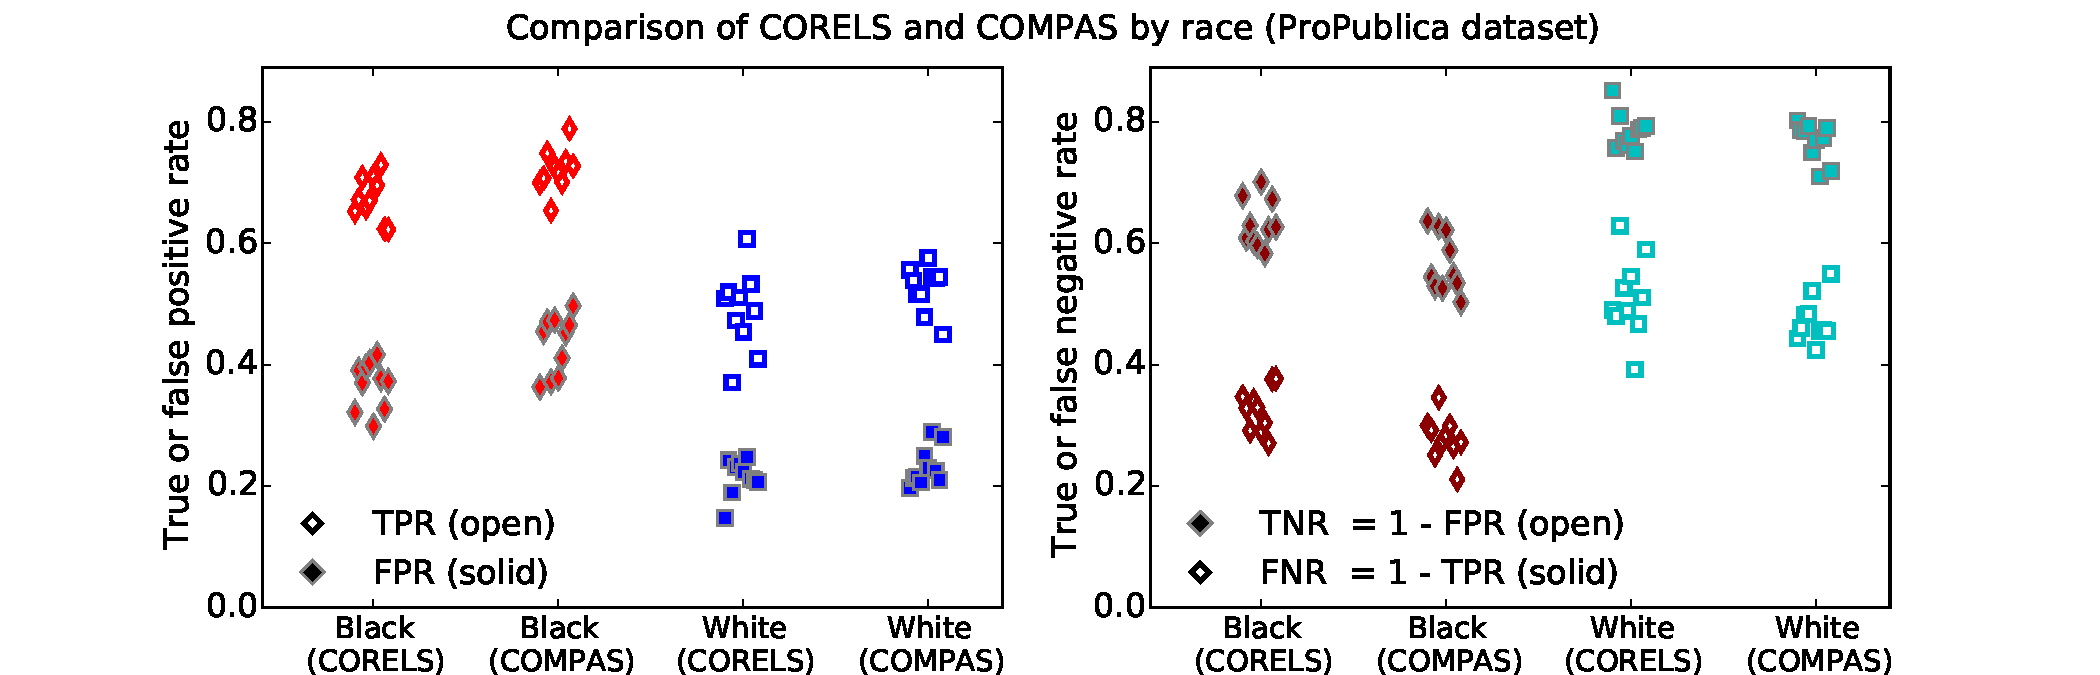
\includegraphics[trim={35mm, 0mm, 40mm, 0mm},
width=0.9\textwidth]{figs/compare_corels_compas.pdf}
\end{center}
\caption{Comparison of TPR and FPR (left), as well as TNR and FNR (right),
for different races in the ProPublica dataset, for CORELS and COMPAS,
across 10 cross-validation folds.
%
%CORELS has a lower FPR for black individuals in the dataset than COMPAS, as well as a lower TPR.
%
%Both CORELS and COMPAS have a significantly higher FPR rate for black indviduals than white individuals--despite CORELS producing optimal rule lists without explicit race features.
%
}
\label{fig:tpr-fpr}
\end{figure}

Figure~\ref{fig:tpr-fpr} shows that CORELS and COMPAS perform similarly across both black and white individuals.
%
Both algorithms have much higher true positive rates (TPR's) and false positive rates (FPR's) for blacks than whites (left), and higher true negative rates (TNR's) and false negative rates (FNR's) for whites than blacks (right).
%
The fact that COMPAS has higher FPR's for blacks and higher FNR's for whites was a central observation motivating ProPublica's claim that COMPAS is racially biased~\citep{LarsonMaKiAn16}.
%
The fact that CORELS' models are so simple, with almost the same results as COMPAS, and do not contain anything except criminal history features and age, indicates possible explanations for the uneven predictions of both COMPAS and CORELS.
%
In particular, blacks tend to have longer criminal histories within the dataset,
(on average, 4.4 crimes for blacks versus~2.6 crimes for whites)
leading to higher FPR's for blacks and higher FNR's for whites.
%
This aspect of the data could entirely explain why ProPublica concluded that COMPAS was racially biased.
%
There are many definitions of fairness, and it is not clear whether CORELS' models are fair either, but it is much easier to debate about the fairness of a model when it is transparent.
%
Additional fairness constraints or transparency constraints can be placed on CORELS' models if desired, though one would need to edit our bounds~(\S\ref{sec:framework}) and implementation~(\S\ref{sec:implementation}) in order to impose more constraints.

Regardless of whether COMPAS is racially biased (which our analysis does not indicate is true as long as criminal history and age are allowed to be considered as features),
COMPAS may have many other fairness defects that might be considered serious.
%
Many of COMPAS's survey questions are direct inquiries about socioeconomic status.
%
For instance, a sample COMPAS survey\footnote{
\url{https://www.documentcloud.org/documents/2702103-Sample-Risk-Assessment-COMPAS-CORE.html}.
Contributed by Julia Angwin, ProPublica.} asks:
``Is it easy to get drugs in your neighborhood?,''
``How often do you have barely enough money to get by?,''
``Do you frequently get jobs that don't pay more than minimum wage?,''
``How often have you moved in the last~12 months?''
%
COMPAS's survey questions also ask about events that were not caused by the person who is being evaluated, such as:
``If you lived with both parents and they later separated, how old were you at the time?,''
``Was one of your parents ever sent to jail or prison?,''
``Was your mother ever arrested, that you know of?"

The fact that COMPAS requires over~130 questions to be answered, many of whose answers may not be verifiable, means that the computation of the COMPAS score is prone to errors.
%
Even the Arnold Foundation's ``public-safety assessment'' (PSA) score -- which is completely transparent, and has only~9 factors -- has been miscalculated in serious criminal trials, leading to a recent lawsuit~\citep{npr-bail:2017}.
%
It is substantially more difficult to obtain the information required to calculate COMPAS scores than PSA scores (with over~14 times the number of survey questions).
%
This significant discrepancy suggests that COMPAS scores are more fallible than PSA scores, as well as even simpler models, like those produced by CORELS.
%
Some of these problems could be alleviated by using only data within electronic records that can be automatically calculated, instead of using information entered by hand and/or collected via subjective surveys.

The United States government pays Northpointe (now called Equivant) to use COMPAS.
%
In light of our observations that CORELS is as accurate as COMPAS on a real-world dataset where COMPAS is used in practice, CORELS predicts similarly to COMPAS for both blacks and whites, and CORELS' models are completely transparent, it is not clear what value COMPAS scores possess.
%
Our experiments also indicate that the proprietary survey data required to compute COMPAS scores has not boosted its prediction accuracy above that of transparent models in practice.

Risk predictions are important for the integrity of the judicial system; judges cannot be expected to keep entire databases in their heads to calculate risks, whereas models (when used correctly) can help to ensure equity.
%
Risk prediction models also have the potential to heavily impact how efficient the judicial system is, in terms of bail and parole decisions; efficiency in this case means that dangerous individuals are not released, whereas non-dangerous individuals are granted bail or parole.
%
High stakes decisions, such as these, are ideal applications for machine learning algorithms that produce transparent models from high dimensional data.

Currently, justice system data does not support highly accurate risk predictions, but current risk models are useful in practice, and these risk predictions will become more accurate as more data and higher quality data are made available.

\subsection{Comparison of CORELS a heuristic model for weapon prediction}
\label{sec:frisk}

CORELS generates simple, accurate models for the task of weapon prediction,
using the NYPD stop-and-frisk dataset.
%
Our approach offers a principled alternative to heuristic models proposed by~\citet{Goel16},
who develop a series of regression models to analyze racial disparities
in New York City's stop-and-frisk policy for a related, larger dataset.
%
In particular, the authors arrive at a heuristic that they suggest
could potentially help police officers more effectively decide when to
frisk and/or search stopped individuals, \ie when such
interventions are likely to discover criminal possession of a weapon (CPW).
%
Starting from a full regression model with~7,705 variables, the authors reduce this to a
smaller model with 98 variables; from this, they keep three variables with the largest coefficients.
%
This gives a heuristic model of the form ${ax + by + cz \ge T}$,
where
\begin{align}
x &= \one[stop~reason = suspicious~object] \nn \\
y &= \one[stop~reason = suspicious~bulge] \nn \\
z &= \one[additional~circumstances = sights~and~sounds~of~criminal~activity], \nn
\end{align}
and~$T$ is a threshold, such that the model predicts CPW when the threshold is met or exceeded.
%
We focus on their approach that uses a single threshold, rather than precinct-specific thresholds.
%
To increase ease-of-use, the authors round the coefficients
to the nearest integers, which gives ${(a, b, c) = (3, 1, 1)}$;
this constrains the threshold to take one of six values, ${T \in \{0, 1, 2, 3, 4, 5\}}$.
%
To employ this heuristic model in the field,
``\dots officers simply need to add at most three small, positive integers \dots
and check whether the sum exceeds a fixed threshold\dots'' \citep{Goel16}.

\begin{figure}[t!]
\begin{center}
% left lower right upper
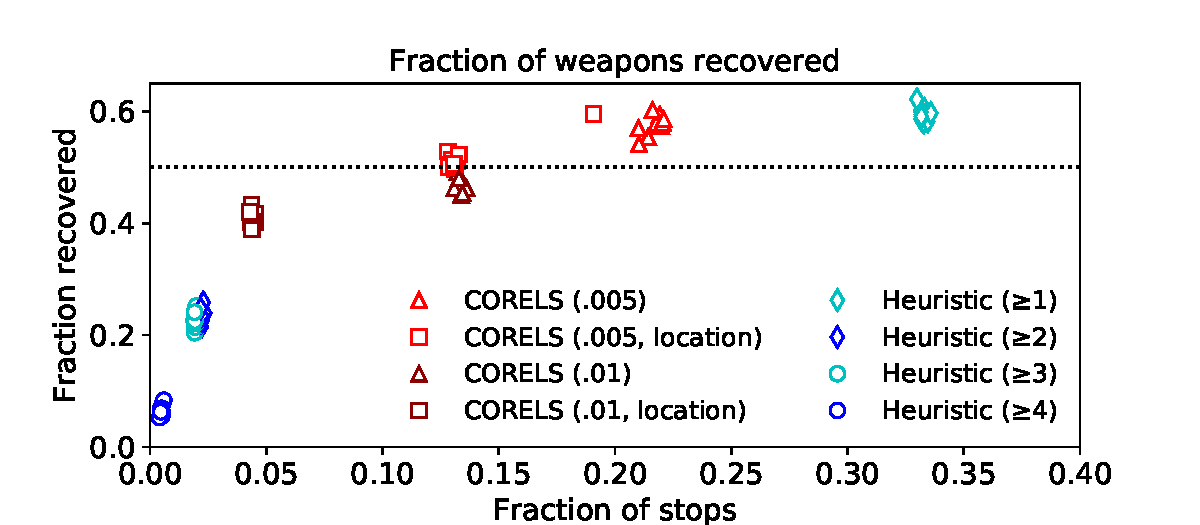
\includegraphics[trim={12mm, 0mm, 24mm, 5mm},
width=0.78\textwidth]{figs/cpw_folds.pdf}
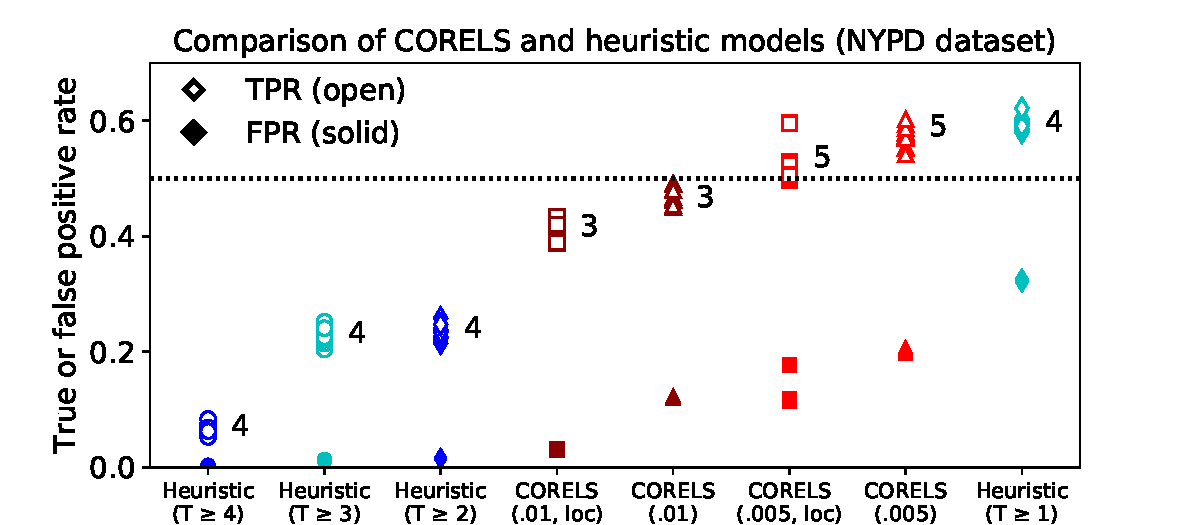
\includegraphics[trim={12mm, 5mm, 24mm, 0mm},
width=0.78\textwidth]{figs/cpw_tpr_fpr.pdf}
\end{center}
\caption{Weapon prediction with the NYPD stop-and-frisk dataset,
for various models learned by CORELS and the heuristic model by~\citet{Goel16},
across~10 cross-validation folds.
%
Note that the fraction of weapons recovered (top) is equal to the TPR (bottom, open markers).
%
Markers above the dotted horizontal lines at the value~0.5 correspond to models that
recover a majority of weapons (that are known in the dataset).
%
Top: Fraction of weapons recovered as a function of the fraction of stops
where the individual was frisked and/or searched.
%
In the legend, entries for CORELS (red markers) indicate the regularization parameter~$(\Reg)$
and whether or not extra location features were used (``location'');
entries for the heuristic model (blue markers) indicate the threshold value~$(T)$.
%
The results we report for the heuristic model
are our reproduction of the results reported in Figure 9 by~\citet{Goel16}
(first four open circles in that figure, from left to right; we exclude the trivial open circle
showing 100\% of weapons recovered at 100\% of stops, obtained by setting the threshold at 0).
%
Bottom: Comparison of TPR (open markers) and FPR (solid markers) for various
CORELS and heuristic models.
%
Models are sorted left-to-right by TPR.
%
Markers and abbreviated horizontal tick labels correspond to the legend in the top~figure.
%
Numbers in the plot label model size; there was no variation in model size across folds,
except for a single fold for CORELS (${\Reg = 0.005}$, Feature Set~C), which found a model of size~6.
}
\label{fig:frisk}
\end{figure}

Figure~\ref{fig:frisk} directly compares various models learned by CORELS to the heuristic models,
using the same dataset as~\citet{Goel16} and 10-fold cross-validation.
%
Recall that we train on resampled data to correct for class imbalance;
we evaluate with respect to test sets that have been formed without resampling.
%
For CORELS, the models correspond to the rule lists illustrated in Figure~\ref{fig:nypd}
from Section~\ref{sec:examples}, and Figures~\ref{fig:cpw-rule-list} and~\ref{fig:cpw-noloc-rule-list}
in Appendix~\ref{appendix:examples}, we consider both Feature Sets~C and~D
and both regularization parameters ${\Reg = 0.005}$ and~0.01.
%
The top panel plots the fraction of weapons recovered as a function of the fraction of
stops where the individual was frisked and/or searched.
%
\citet{Goel16} target models that efficiently recover a majority of weapons
(while also minimizing racial disparities, which we do not address here).
%
Interestingly, the models learned by CORELS span a significant region that is not available
to the heuristic model, which would require larger or non-integer parameters to access the region.
%
The region is possibly desirable, since it includes models (${\Reg = 0.005}$, bright red)
that recover a majority (${\ge 50\%}$) of weapons (that are known in the dataset).
%
More generally, CORELS' models all recover at least ${40\%}$ of weapons
on average, \ie more weapons than any of the heuristic models with~${T \ge 2}$,
which recover less than 25\% of weapons on average.
%
At the same time, CORELS' models all require well under 25\% of stops---significantly
less than the heuristic model with~${T = 1}$, which requires over 30\% of stops
to recover a fraction of weapons comparable to the CORELS model that recovers the most weapons.

The bottom panel in Figure~\ref{fig:frisk} plots both TPR and FPR and labels model size,
for each of the models in the top panel.
%
For the heuristic, we define model size as the number of model parameters;
for CORELS, we use the number of rules in the rule list,
which is equal to the number of leaves when we view a rule list as a decision tree.
%
The heuristic models all have~4 parameters, while the different CORELS models have
either~3 or approximately~5 rules.
%
CORELS' models are thus approximately as small, interpretable, and transparent
as the heuristic models; furthermore, their predictions are straightforward
to compute, without even requiring arithmetic.

\subsection{Predictive performance and model size for CORELS and other algorithms}
\label{sec:sparsity}

\begin{figure}[t!]
\begin{center}
%\includegraphics[width=0.75\textwidth]{figs/sketch-comparison.png}
% left lower right upper
%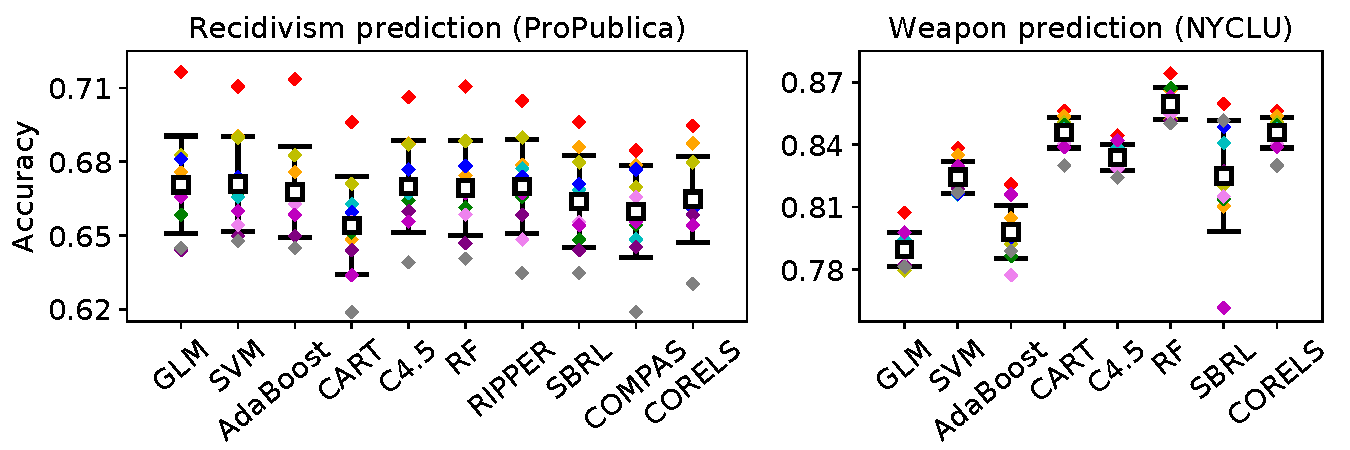
\includegraphics[trim={2mm, 10mm, 2mm, 0mm}, width=\textwidth]{figs/compare-compas-weapon.pdf}
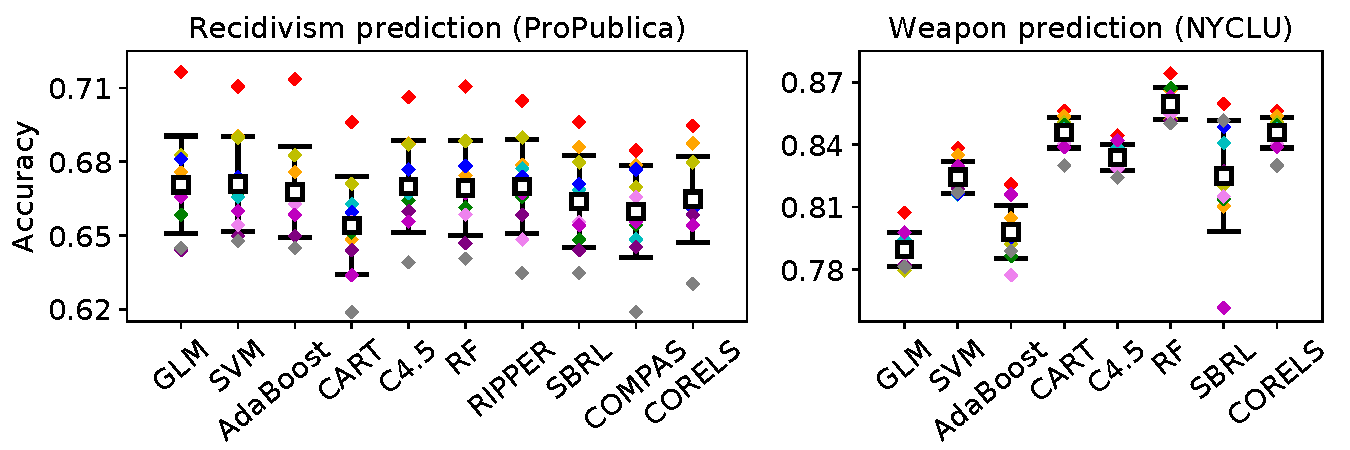
\includegraphics[trim={2mm, 5mm, 102mm, 0mm}, clip,
width=0.5\textwidth]{figs/compare-compas-weapon.pdf}
\end{center}
\caption{Two-year recidivism prediction for the ProPublica COMPAS dataset.
%
Comparison of CORELS and a panel of eight other algorithms:
logistic regression~(GLM), support vector machines~(SVM),
AdaBoost, CART, C4.5, random forests~(RF), RIPPER,
scalable Bayesian rule lists~(SBRL).
%
For CORELS, we use regularization parameter~${\Reg=0.005}$.
}
\label{fig:compas-comparison}
\end{figure}

We ran a 10-fold cross validation experiment using CORELS
and eight other algorithms:
logistic regression, support vector machines (SVM), AdaBoost, CART, C4.5,
random forest (RF), RIPPER, and scalable Bayesian rule lists (SBRL).\footnote{For
SBRL, we use the C implementation at \url{https://github.com/Hongyuy/sbrlmod}.
By default, SBRL sets ${\eta = 3}$, ${\lambda = 9}$,
the number of chains to 11 and iterations to 1,000.}
%
We use standard R packages, with default parameter settings,
for the first seven algorithms.\footnote{For CART, C4.5 (J48), and RIPPER,
we use the R packages rpart, RWeka, and caret, respectively.
%
By default, CART uses complexity parameter ${cp = 0.01}$ and C4.5 uses complexity parameter ${C = 0.25}$.
}
%
We use the same antecedent sets as input to the two rule list learning algorithms, CORELS and SBRL;
for the other algorithms, the inputs are binary feature sets corresponding to the
single clause antecedents in the aforementioned antecedent sets (see Appendix~\ref{appendix:data}).

Figure~\ref{fig:compas-comparison} shows that for the ProPublica dataset,
there were no statistically significant differences in test accuracies across algorithms;
the difference between folds was far larger than the difference between algorithms.
%
Figure~\ref{fig:weapon-comparison} shows that for the NYCLU dataset,
logistic regression, SVM, and AdaBoost have the highest TPR's and also the highest FPR's;
we show TPR and FPR due to class imbalance.
%
For this problem, CORELS obtains an intermediate TPR, compared to other algorithms,
while achieving a relatively low FPR.
%
We conclude that CORELS produces models whose predictive performance is comparable to or better than
those found via other algorithms.

\begin{figure}[t!]
\begin{center}
%\includegraphics[width=0.75\textwidth]{figs/sketch-comparison.png}
% left lower right upper
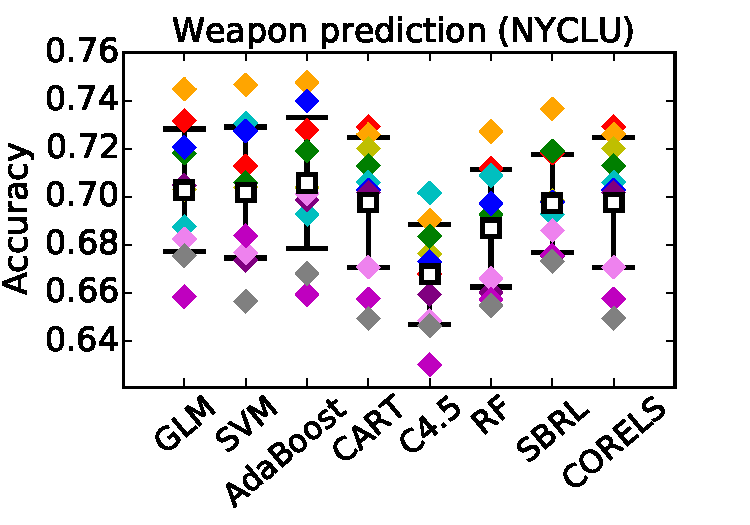
\includegraphics[trim={2mm, 10mm, 2mm, 0mm},
width=\textwidth]{figs/compare-weapon.pdf}
\end{center}
\caption{TPR (left) and FPR (right) for the test set,
for CORELS and a panel of seven other algorithms,
for the weapon prediction problem with the NYCLU stop-and-frisk dataset.
%
Means (white squares),
standard deviations (error bars),
and values (colors correspond to folds),
for 10-fold cross-validation experiments.
%
For CORELS, we use~${\Reg=0.01}$.
%
Note that we were unable to execute RIPPER for the NYCLU problem.
}
\label{fig:weapon-comparison}
\end{figure}
%
\begin{figure}[t!]
\begin{center}
%\includegraphics[width=0.75\textwidth]{figs/sketch-comparison.png}
% left lower right upper
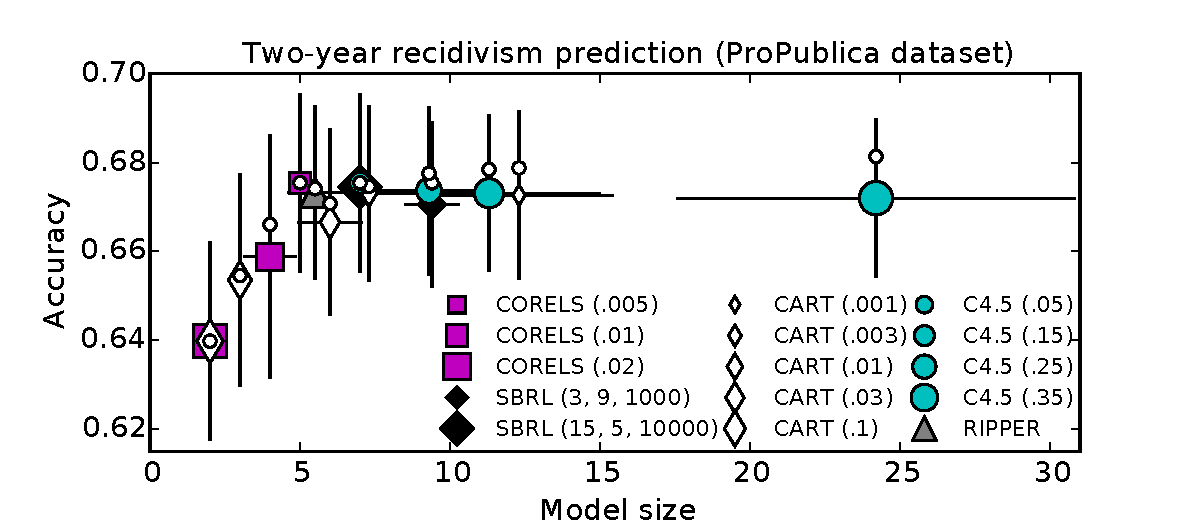
\includegraphics[trim={12mm, 5mm, 24mm, 5mm},
width=0.78\textwidth]{figs/compas-sparsity-training.pdf}
%
\end{center}
\caption{Training and test accuracy as a function of model size, across different methods,
for two-year recidivism prediction with the ProPublica COMPAS dataset.
%
In the legend, numbers in parentheses are algorithm parameters that we vary
for CORELS~($\Reg$), CART~($cp$), C4.5~($C$), and SBRL ($\eta$, $\lambda$, $i$),
where~$i$ is the number of iterations.
%
Legend markers and error bars indicate means and standard deviations,
respectively, across cross-validation folds.
%
Small circles mark training accuracy means.
%
None of the models exhibit significant overfitting;
mean training accuracy never exceeds mean test accuracy
by more than about 0.01.
}
\label{fig:sparsity-compas}
\end{figure}

Figures~\ref{fig:sparsity-compas} and~\ref{fig:sparsity-weapon} summarize differences
in predictive performance and model size
for CORELS and other tree (CART, C4.5) and rule list (RIPPER, SBRL) learning algorithms.
%
Here, we vary different algorithm parameters, and increase the number of iterations for SBRL to 10,000.
%
For two-year recidivism prediction with the ProPublica dataset (Figure~\ref{fig:sparsity-compas}),
we plot both training and test accuracy,
as a function of the number of leaves in the learned model.
%
Due to class imbalance for the weapon prediction problem with the NYCLU stop-and-frisk dataset
(Figure~\ref{fig:sparsity-weapon}), we plot both true positive rate (TPR) and false positive rate (FPR),
again as a function of the number of leaves.
%
For both problems, CORELS can learn short rule lists without sacrificing predictive performance.
%
For listings of example optimal rule lists that correspond to the results
for CORELS summarized here, see Appendix~\ref{appendix:examples}.
%
Also see Figure~\ref{fig:sparsity-cpw} in Appendix~\ref{appendix:cpw}; it uses the larger
NYPD dataset and is similar to Figure~\ref{fig:sparsity-weapon}.

\begin{figure}[t!]
\begin{center}
%\includegraphics[width=0.75\textwidth]{figs/sketch-comparison.png}
% left lower right upper
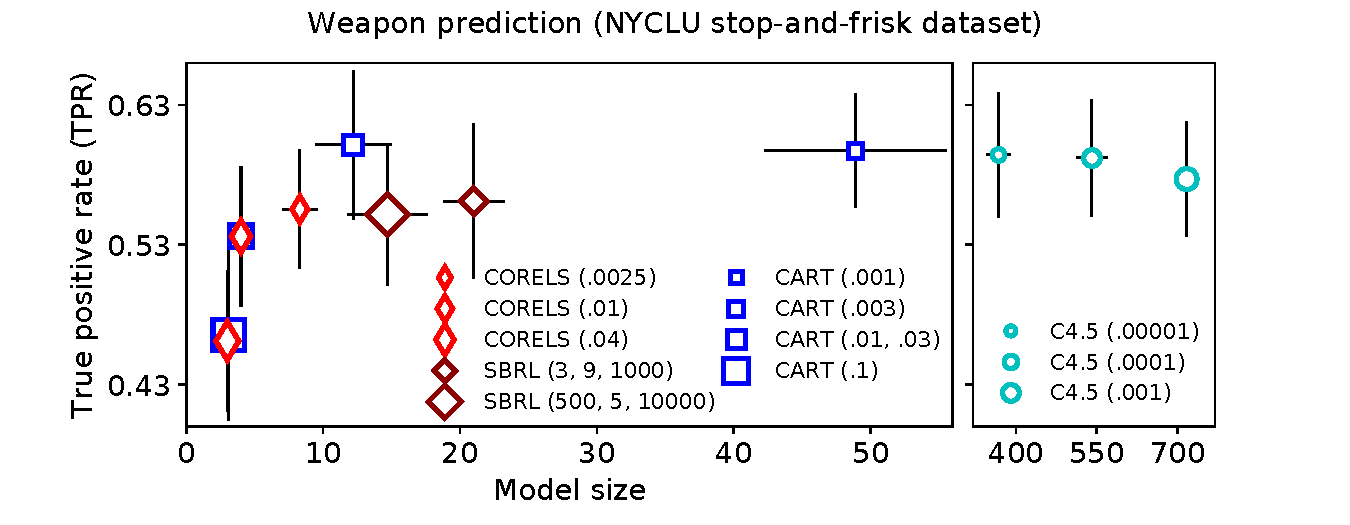
\includegraphics[trim={17mm, 0mm, 27mm, 0mm},
width=0.78\textwidth]{figs/weapon-sparsity-tpr.pdf}
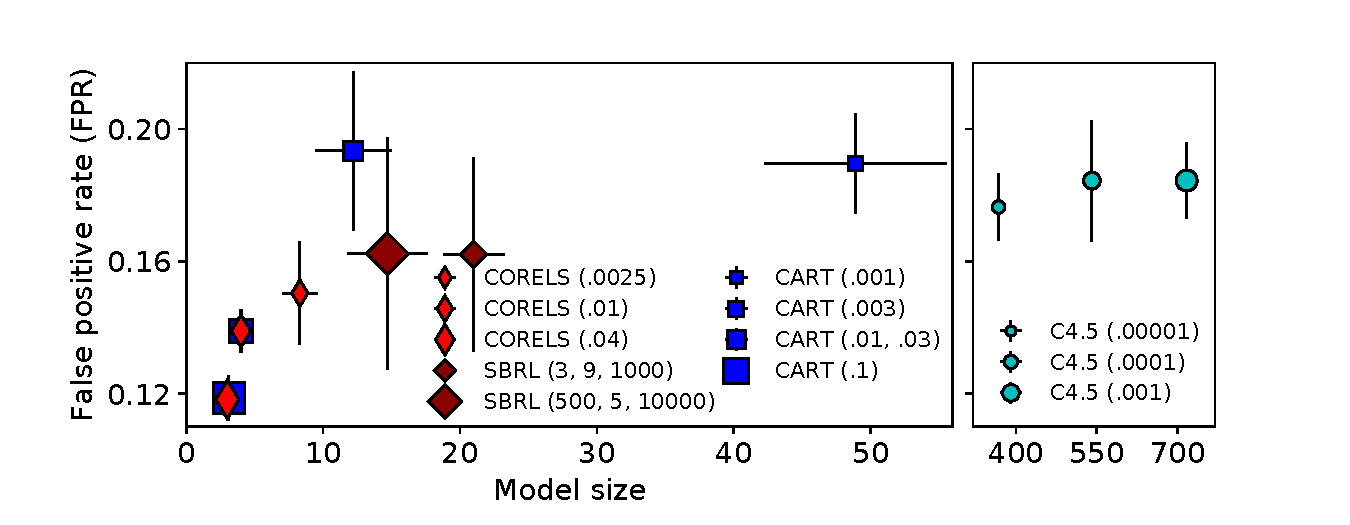
\includegraphics[trim={17mm, 10mm, 27mm, 4mm},
width=0.78\textwidth]{figs/weapon-sparsity-fpr.pdf}
\end{center}
\caption{TPR (top) and FPR (bottom)
for the test set, as a function of model size, across different methods,
for weapon prediction with the NYCLU stop-and-frisk dataset.
%
In the legend, numbers in parentheses are algorithm parameters,
as in Figure~\ref{fig:sparsity-compas}.
%
Legend markers and error bars indicate means and standard deviations,
respectively, across cross-validation folds.
%
%For CORELS and SBRL, we use ${M = 28}$ antecedents.
%
%CART with ${cp = 0.001}$ significantly overfits;
%C4.5 finds large models and dramatically overfits for all tested parameters.
C4.5 finds large models for all tested parameters.
}
\label{fig:sparsity-weapon}
\end{figure}

\subsection{CORELS execution traces, for different regularization parameters}
\label{sec:reg-param}
In this section, we illustrate several views of CORELS execution traces,
for the NYCLU stop-and-frisk dataset with ${M = 46}$ antecedents,
for the same three regularization parameters (${\Reg = .04, .01, .025}$)
as in Figure~\ref{fig:sparsity-weapon}.

\begin{table}[t!]
\centering
%\begin{centering}
CORELS with different regularization parameters (NYCLU stop-and-frisk dataset) \\
%\end{centering}
\vspace{2mm}
\begin{tabular}{l | c | c | c | c}
& Total & Time to & Max evaluated & Optimal \\
$\lambda$ & time (s) & optimum (s) & prefix length & prefix length \\
\hline
.04 & .61 (.03) & .002 (.001) & 6 & 2 \\
.01 & 70 (6) & .008 (.002) & 11 & 3 \\
.0025 & 1600 (100) & 56 (74) & 16-17 & 6-10 \\
\hline
\end{tabular}
\begin{tabular}{l | c | c | c}
\hline
& Lower bound & Total queue &  Max queue \\
$\lambda$ &~ evaluations ($\times 10^6$) ~&~ insertions ($\times 10^3$) ~&~ size ($\times 10^3$) \\
\hline
.04 & .070 (.004) & 2.2 (.1) & .9 (.1) \\
.01 & 7.5 (.6) & 210 (20) & 130 (10) \\
.0025 & 150 (10) & 4400 (300) & 2500 (170) \\
\end{tabular}
%\vspace{4mm}
\caption{Summary of CORELS executions, for the NYCLU stop-and-frisk dataset (${M = 46}$),
for same three regularization parameter ($\Reg$) values as in Figure~\ref{fig:sparsity-weapon}.
%
The columns report the total execution time,
time to optimum, maximum evaluated prefix length, optimal prefix length,
number of times we completely evaluate a prefix~$\Prefix$'s lower bound~$b(\Prefix, \x, \y)$,
total number of queue insertions (this number is equal to the number of cache insertions),
and the maximum queue size.
%
For prefix lengths, we report single values or ranges corresponding to the minimum and maximum observed values;
in the other columns, we report means (and standard deviations) over 10 cross-validation folds.
%
See also Figures~\ref{fig:weapon-reg-execution} and~\ref{fig:queue-weapon-reg}.
}
\vspace{4mm}
\label{tab:weapon-reg}
\end{table}

Table~\ref{tab:weapon-reg} summarizes execution traces across all 10 cross-validation folds.
%
For each value of~$\Reg$, CORELS achieves the optimum in a small fraction of the total execution time.
%
As~$\Reg$ decreases, these times increase because the search problems become more difficult,
as is summarized by the observation that CORELS must evaluate longer prefixes;
consequently, our data structures grow in size.
%
We report the total number of elements inserted into the queue and the maximum queue size;
recall from~\S\ref{sec:implementation} that the queue elements correspond to the trie's leaves,
and that the symmetry-aware map elements correspond to the trie's nodes.

\begin{figure}[t!]
\begin{center}
% left lower right upper
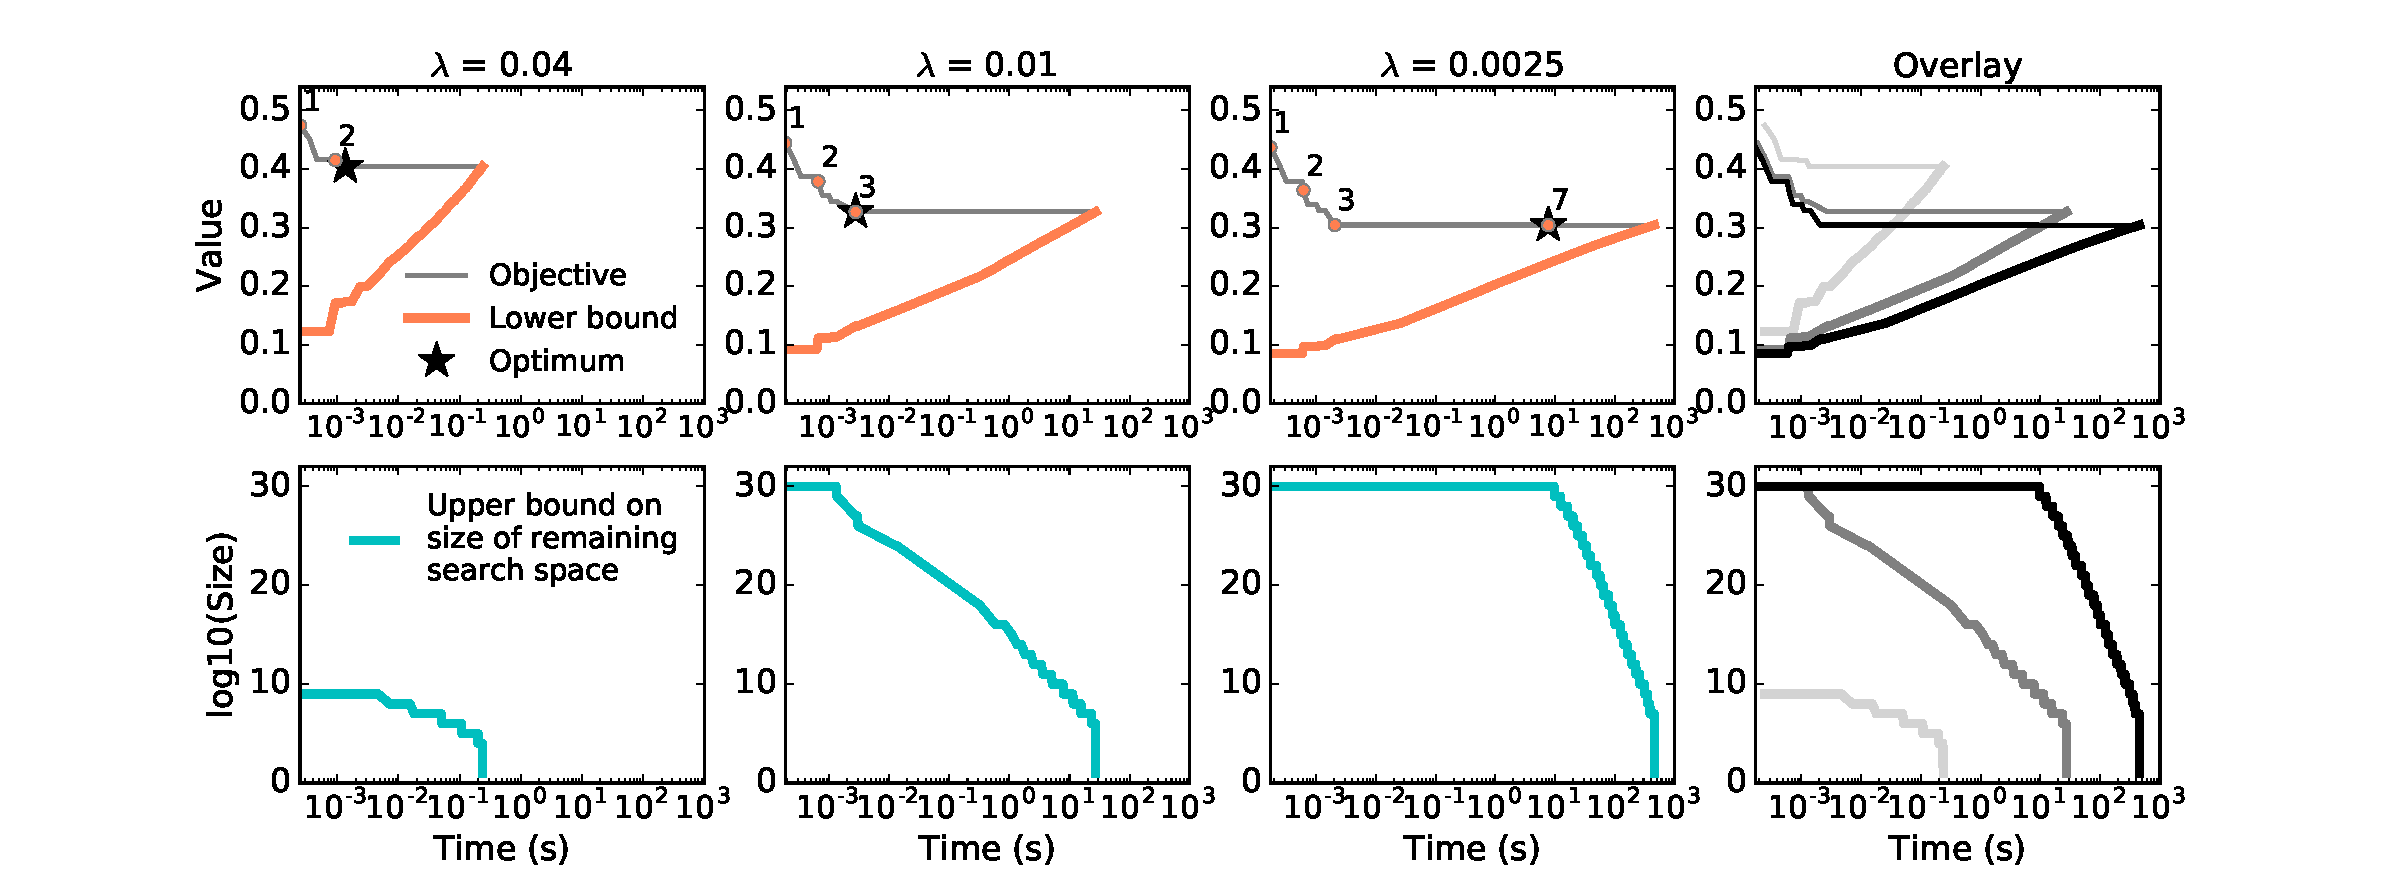
\includegraphics[trim={35mm 0mm 35mm 15mm},
width=0.92\textwidth]{figs/weapon_reg-execution.pdf}
\end{center}
\vspace{-5mm}
\caption{Example executions of CORELS, for the NYCLU stop-and-frisk dataset (${M = 46}$).
%
See also Table~\ref{tab:weapon-reg} and Figure~\ref{fig:queue-weapon-reg}.
%
Top: Objective value (solid line) and lower bound (dashed line) for CORELS,
as a function of wall clock time (log scale).
%
Numbered points along the trace of the objective value
indicate when the length of the best known rule list changes
and are labeled by the new length.
%
For each value of~$\Reg$, a star marks the optimum objective value
and time at which it was achieved.
%
Bottom: $\lfloor \log_{10} \Remaining(\CurrentObj, \Queue) \rfloor$,
as a function of wall clock time (log scale),
where~$\Remaining(\CurrentObj, \Queue)$
is the upper bound on remaining search space size
(Theorem~\ref{thm:remaining-eval-fine}).
%
Rightmost panels: For visual comparison, we overlay the execution traces
from the panels to the left, for the three different values of~$\Reg$.
}
\label{fig:weapon-reg-execution}
\end{figure}
%
\begin{figure}[t!]
\begin{center}
% left lower right upper
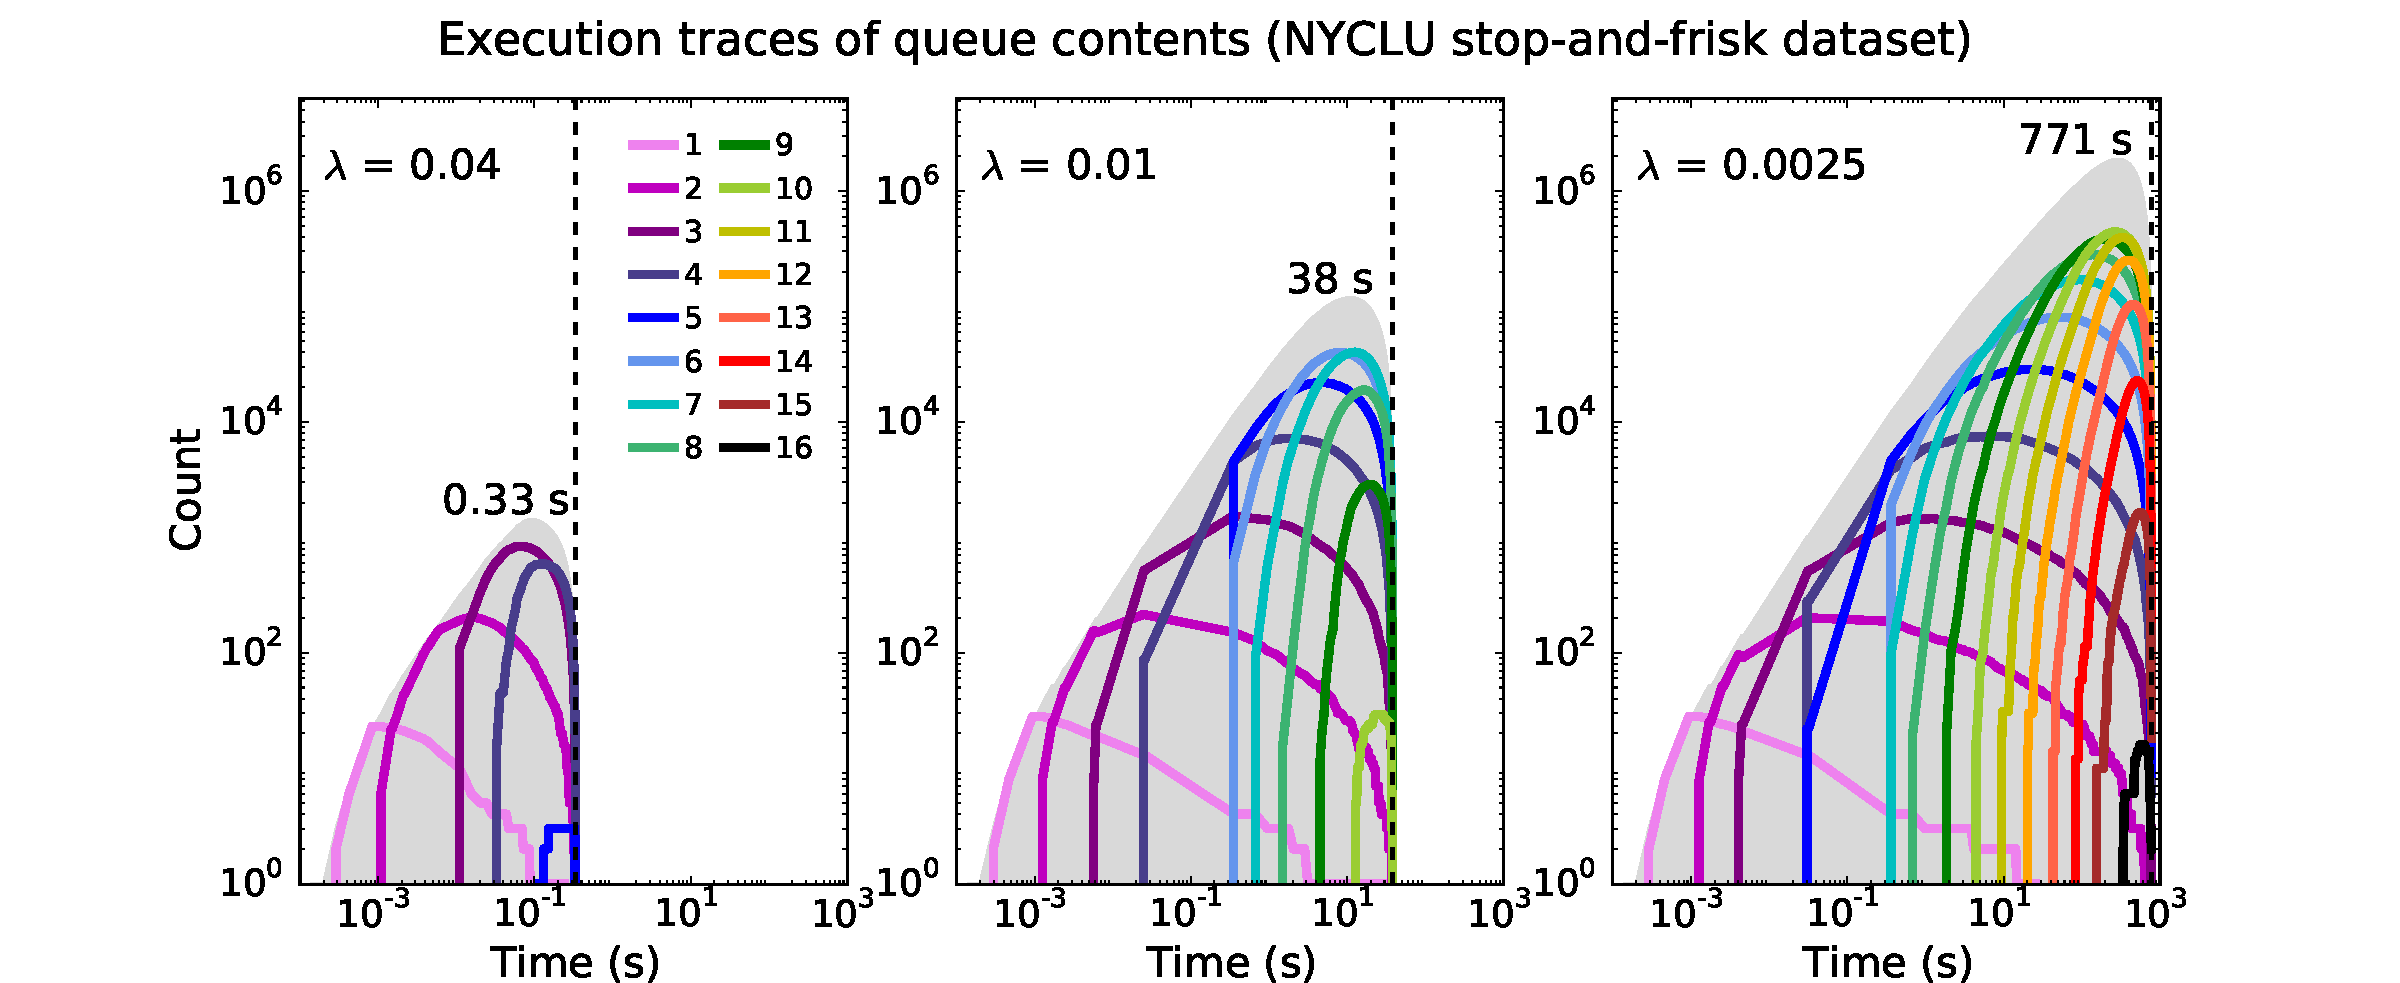
\includegraphics[trim={30mm 0mm 30mm 3mm},
width=0.92\textwidth]{figs/weapon_reg-queue.pdf}
\end{center}
\vspace{-5mm}
\caption{Summary of CORELS' logical queue,
%\ie the nodes in the physical queue that have not been marked for deletion,
for the NYCLU stop-and-frisk dataset (${M = 46}$),
for same three regularization parameters as in Figure~\ref{fig:sparsity-weapon}
and Table~\ref{tab:weapon-reg}.
%
Solid lines plot the numbers of prefixes in the logical queue (log scale), colored by length (legend),
as a function of wall clock time (log scale).
%
All plots are generated using a single, representative cross-validation training set.
%
For each execution, the gray shading fills in the area beneath the total number
of queue elements, \ie the sum over all lengths;
we also annotate the total time in seconds, marked with a dashed vertical line.
}
\label{fig:queue-weapon-reg}
\end{figure}

The upper panels in Figure~\ref{fig:weapon-reg-execution} plot example execution traces,
from a single cross-validation fold, of both the current best objective value~$\CurrentObj$
and the lower bound~$b(\Prefix, \x, \y)$ of the prefix~$\Prefix$ being evaluated.
%
These plots illustrate that CORELS certifies optimality
when the lower bound matches the objective value.
%
The lower panels in Figure~\ref{fig:weapon-reg-execution} plot corresponding traces of
an upper bound on the size of the remaining search space (Theorem~\ref{thm:remaining-eval-fine}),
and illustrate that as~$\Reg$ decreases, it becomes more difficult to eliminate regions of the search~space.
%
For Figure~\ref{fig:weapon-reg-execution}, we dynamically and incrementally
calculate~$\lfloor \log_{10} \Remaining(\CurrentObj, \Queue) \rfloor$,
which adds some computational overhead; we do not calculate this elsewhere unless noted.

Figure~\ref{fig:queue-weapon-reg} visualizes the elements in CORELS' logical queue,
for each of the executions in Figure~\ref{fig:weapon-reg-execution}.
%
Recall from~\S\ref{sec:gc} that the logical queue corresponds to elements in the
(physical) queue that have not been garbage collected from the trie; these are prefixes that
CORELS has already evaluated and whose children the algorithm plans to evaluate next.
%
As an execution progresses, longer prefixes are placed in the queue;
as~$\Reg$ decreases, the algorithm must spend more time evaluating longer and longer prefixes.

%\newpage
\subsection{Efficacy of CORELS algorithm optimizations}
\label{sec:ablation}

%\includegraphics[width=0.75\textwidth]{figs/sketch-ablation.png}
\begin{table}[t!]
\centering
%\begin{centering}
Per-component performance improvement (ProPublica dataset) \\
%\end{centering}
\vspace{1mm}
\begin{tabular}{l | c  r | c | c}
& Total time & Slow- & Time to & Max evaluated \\
Algorithm variant & (min) & down & optimum (s) & prefix length \\
\hline
CORELS & 0.98 (.6) & --- & 1 (1) & 5 \\
No priority queue (BFS) & 1.03 (.6) & 1.1$\times$ & 2 (4) & 5 \\
No support bounds & 1.5 (.9) & 1.5$\times$ & 1 (2) & 5 \\
No lookahead bound & 12.3 (6.2) & 13.3$\times$ & 1 (1) & 6 \\
No symmetry-aware map & 9.1 (6.4) & 8.4$\times$ & 2 (3) & 5 \\
No equivalent points bound* & $>$130 (2.6) & $>$180$\times$ & $>$1400 (2000) & $\ge$11 \\
\hline
\end{tabular}
\begin{tabular}{l | c | c | c}
\hline
 & Lower bound & Total queue &  Max queue \\
Algorithm variant & evaluations ($\times 10^6$) & insertions ($\times 10^6$) &~ size ($\times 10^6$) \\
\hline
CORELS & 26 (15) & .29 (.2) & .24 (.1) \\
No priority queue (BFS) & 27 (16) & .33 (.2) & .20 (.1) \\
No support bounds & 42 (25) & .40 (.2) & .33 (.2) \\
No lookahead bound & 320 (160) & 3.6 (1.8) & 3.0 (1.5) \\
No symmetry-aware map & 250 (180) & 2.5 (1.7) & 2.4 (1.7) \\
No equivalent points bound* & $>$940 (5) & $>$510 (1.1) & $>$500 (1.2) \\
\end{tabular}
%\vspace{4mm}
\caption{Per-component performance improvement, for the ProPublica dataset
(${\Reg = 0.005}$, ${M = 122}$).
%
The columns report the total execution time,
time to optimum, maximum evaluated prefix length,
number of times we completely evaluate a prefix~$\Prefix$'s lower bound~$b(\Prefix, \x, \y)$,
total number of queue insertions (which is equal to the number of cache insertions),
and maximum logical queue size.
%
The first row shows CORELS; subsequent rows show variants
that each remove a specific implementation optimization or bound.
%
(We are not measuring the cumulative effects of removing a sequence of components.)
%
All rows represent complete executions that certify optimality,
except those labeled `No equivalent points bound,'
for which each execution was terminated due to memory constraints,
once the size of the cache reached ${5 \times 10^8}$ elements,
after consuming $\sim$250GB RAM.
%
In all but the final row and column, we report means
(and standard deviations) over 10 cross-validation folds.
%
We also report the  mean slowdown in total execution time,
with respect to CORELS.
%
In the final row, we report the mean (and standard deviation) of the
incomplete execution time and corresponding slowdown,
and a lower bound on the mean time to optimum;
in the remaining fields, we report minimum values across folds.
%
See also Figure~\ref{fig:queue}. \\
%
*~Only 7 out of 10 folds achieve the optimum before being terminated.
}
\vspace{4mm}
\label{tab:ablation}
\end{table}

This section examines the efficacy of each of our bounds and data structure optimizations.
%
We remove a single bound or data structure optimization from our final implementation and measure
how the performance of our algorithm changes.
%
We examine these performance traces on both the NYCLU and the ProPublica datasets,
and highlight the result that on different problems, the relative performance improvements
of our optimizations can vary.

\begin{figure}[t!]
\begin{center}
% left lower right upper
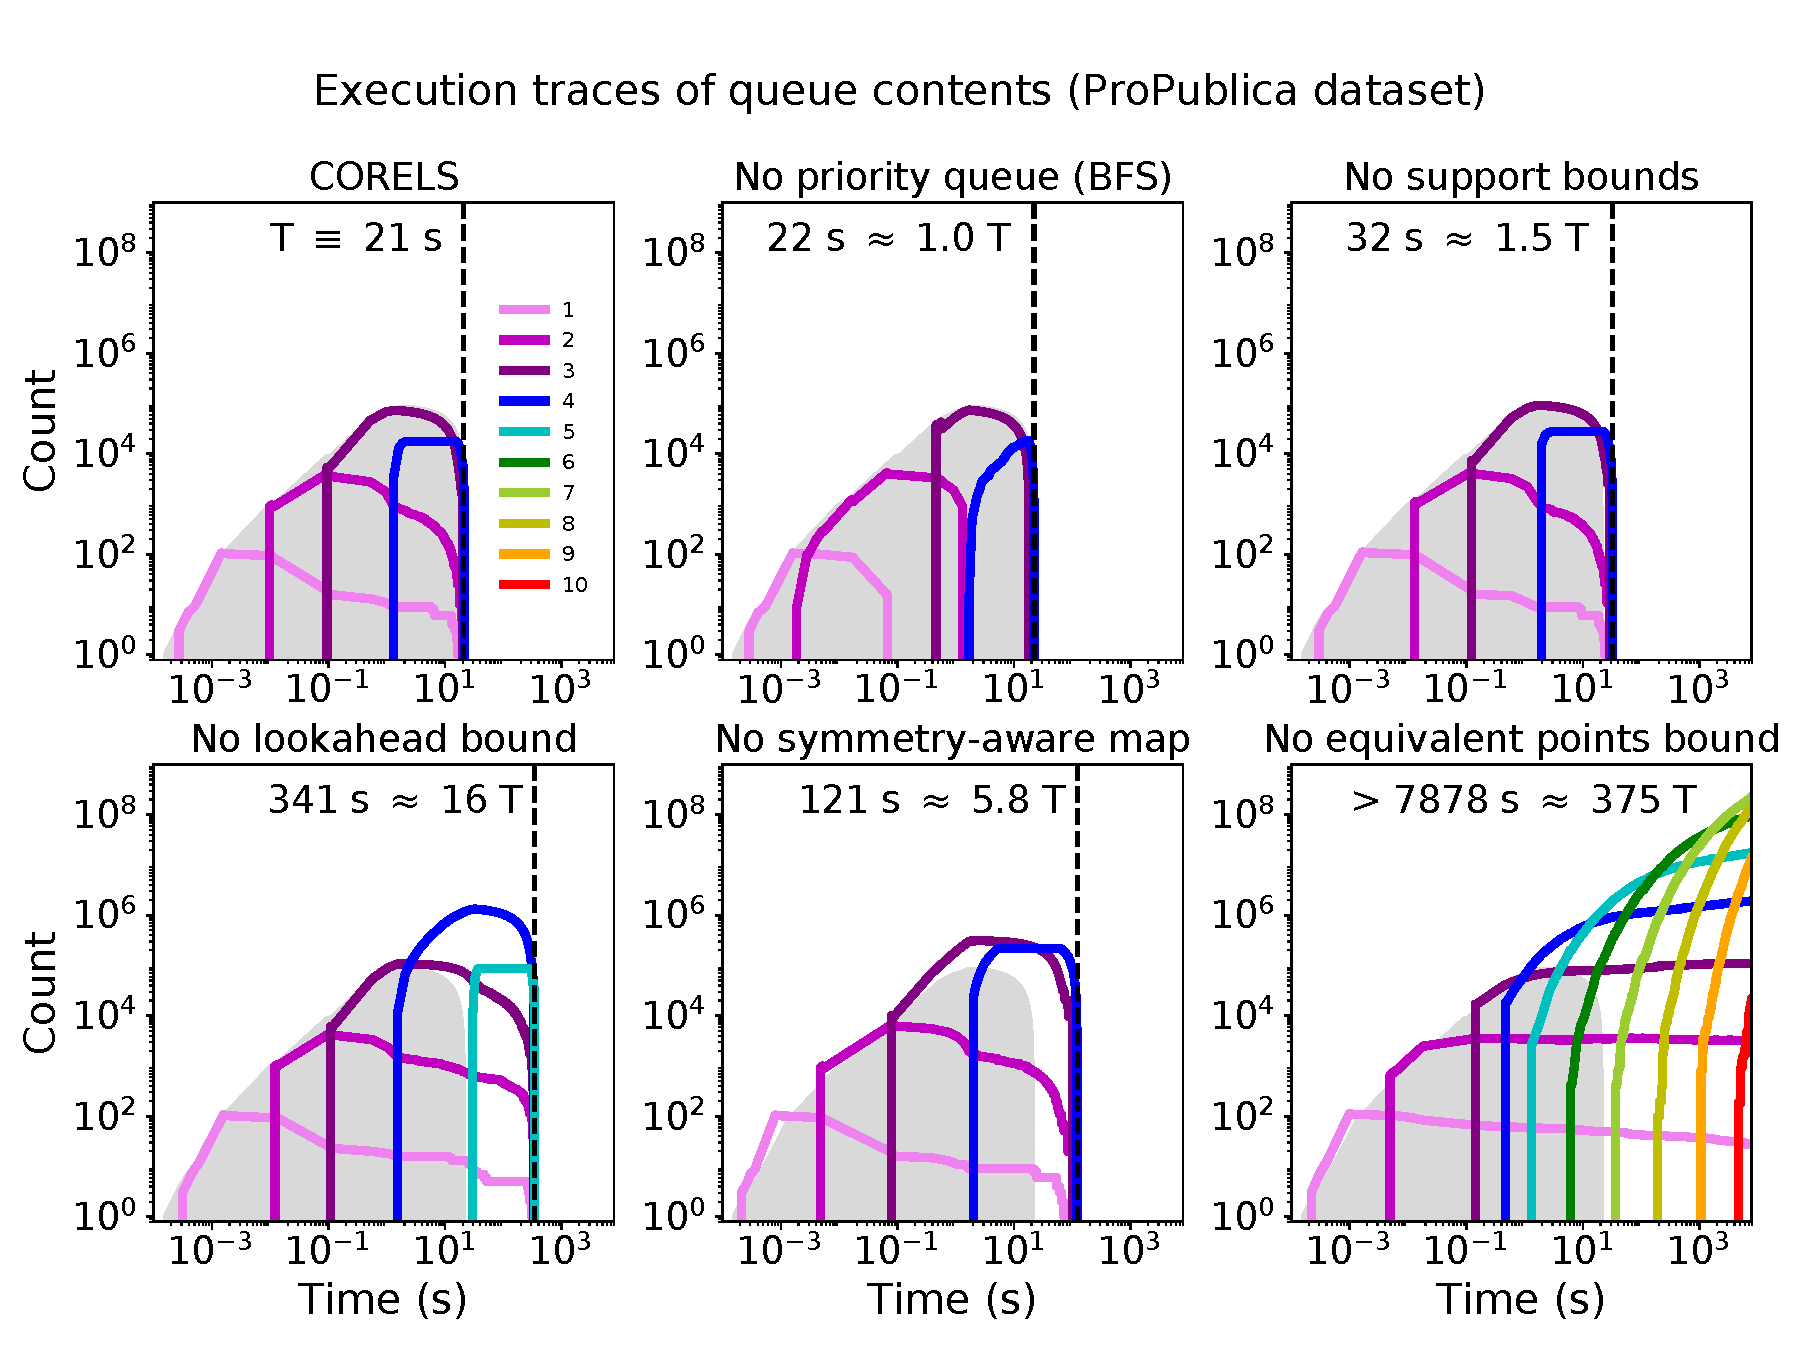
\includegraphics[trim={0mm 0mm 0mm 15mm}, width=\textwidth]{figs/jmlr_compas_ablation-queue.pdf}
\end{center}
\vspace{-5mm}
\caption{Summary of the logical queue's contents, for full CORELS (top left)
%\ie the nodes in the physical queue that have not been marked for deletion,
and five variants that each remove a specific implementation optimization or bound,
for the ProPublica dataset (${\Reg = 0.005}$, ${M = 122}$).  See also Table~\ref{tab:ablation}.
%
Solid lines plot the numbers of prefixes in the logical queue (log scale), colored by length (legend),
as a function of wall clock time (log scale).
%
All plots are generated using a single, representative cross-validation training set.
%
The gray shading fills in the area beneath the total number of
queue elements for CORELS,
\ie the sum over all lengths in the top left figure.
%
For comparison, we replicate the same gray region
in the other five subfigures.
%
For each execution, we indicate the total time in seconds,
relative to the full CORELS implementation (T = 21 s),
and with a dashed vertical line.
%
The execution without the equivalent points bound (bottom right) is incomplete.
}
\label{fig:queue}
\end{figure}

Table~\ref{tab:ablation} provides summary statistics for experiments using the full
CORELS implementation (first row) and five variants (subsequent rows) that each remove a specific optimization:
%
(1)~Instead of a priority queue (\S\ref{sec:queue}) ordered by the objective lower bound,
we use a queue that implements breadth-first search (BFS).
%
(2)~We remove checks that would trigger pruning via
our lower bounds on antecedent support (Theorem~\ref{thm:min-capture})
and accurate antecedent support (Theorem~\ref{thm:min-capture-correct}).
%
(3)~We remove the effect of our lookahead bound (Lemma~\ref{lemma:lookahead}),
which otherwise tightens the objective lower bound by an amount equal to the regularization parameter~$\Reg$.
%
(4)~We disable the symmetry-aware map (\S\ref{sec:pmap}), our data structure
that enables pruning triggered by the permutation bound (Corollary~\ref{thm:permutation}).
%
(5)~We do not identify sets of equivalent points, which we otherwise use to tighten the
objective lower bound via the equivalent points bound (Theorem~\ref{thm:identical}).

\begin{table}[t!]
\centering
%\begin{centering}
Per-component performance improvement (NYCLU stop-and-frisk dataset) \\
%\end{centering}
\vspace{1mm}
\begin{tabular}{l | c  r | c | c}
& Total & Slow- & Time to & Max evaluated \\
Algorithm variant & time (min) & down & optimum ($\mu$s) & prefix length \\
\hline
CORELS & 1.1 (.1) & --- & 8.9 (.1) & 11 \\
No priority queue (BFS) & 2.2 (.2) & 2.0$\times$ & 110 (10) & 11 \\
No support bounds & 1.2 (.1) & 1.1$\times$ & 8.8 (.8) & 11 \\
No lookahead bound & 1.7 (.2) & 1.6$\times$ & 7.3 (1.8) & 11-12 \\
No symmetry-aware map & $>$ 73 (5) & $>$ 68$\times$ & $>$ 7.6 (.4) & $>$ 10 \\
No equivalent points bound & 4 (.3) & 3.8$\times$ & 6.4 (.9) & 14 \\
\hline
\end{tabular}
\begin{tabular}{l | c | c | c}
\hline
 & Lower bound & Total queue &  Max queue \\
Algorithm variant & evaluations ($\times 10^6$) & insertions ($\times 10^5$) &~ size ($\times 10^5$) \\
\hline
CORELS & 7 (1) & 2.0 (.2) & 1.3 (.1) \\
No priority queue (BFS) & 14 (1) & 4.1 (.4) & 1.4 (.1) \\
No support bounds & 8 (1) & 2.1 (.2) & 1.3 (.1) \\
No lookahead bound & 11 (1) & 3.2 (.3) & 2.1 (.2) \\
No symmetry-aware map & $>$ 390 (40) & $>$ 1000 (0) & $>$ 900 (10) \\
No equivalent points bound & 33 (2) & 9.4 (.7) & 6.0 (.4) \\
\end{tabular}
%\vspace{4mm}
\caption{Per-component performance improvement, as in Table~\ref{tab:ablation},
for the NYCLU stop-and-frisk dataset (${\Reg = 0.01}$, ${M = 46}$).
%
All rows except those labeled `No symmetry-aware map' represent complete executions.
%
A single fold running without a symmetry-aware map required over 2 days to complete,
so in order to run all 10 folds above, we terminated execution after the prefix tree~(\S\ref{sec:trie})
reached~$10^8$ nodes.
%
See Table~\ref{tab:ablation} for a detailed caption,
and also Figure~\ref{fig:queue-weapon}.
}
\vspace{4mm}
\label{tab:ablation-weapon}
\end{table}
%
\begin{figure}[t!]
\begin{center}
% left lower right upper
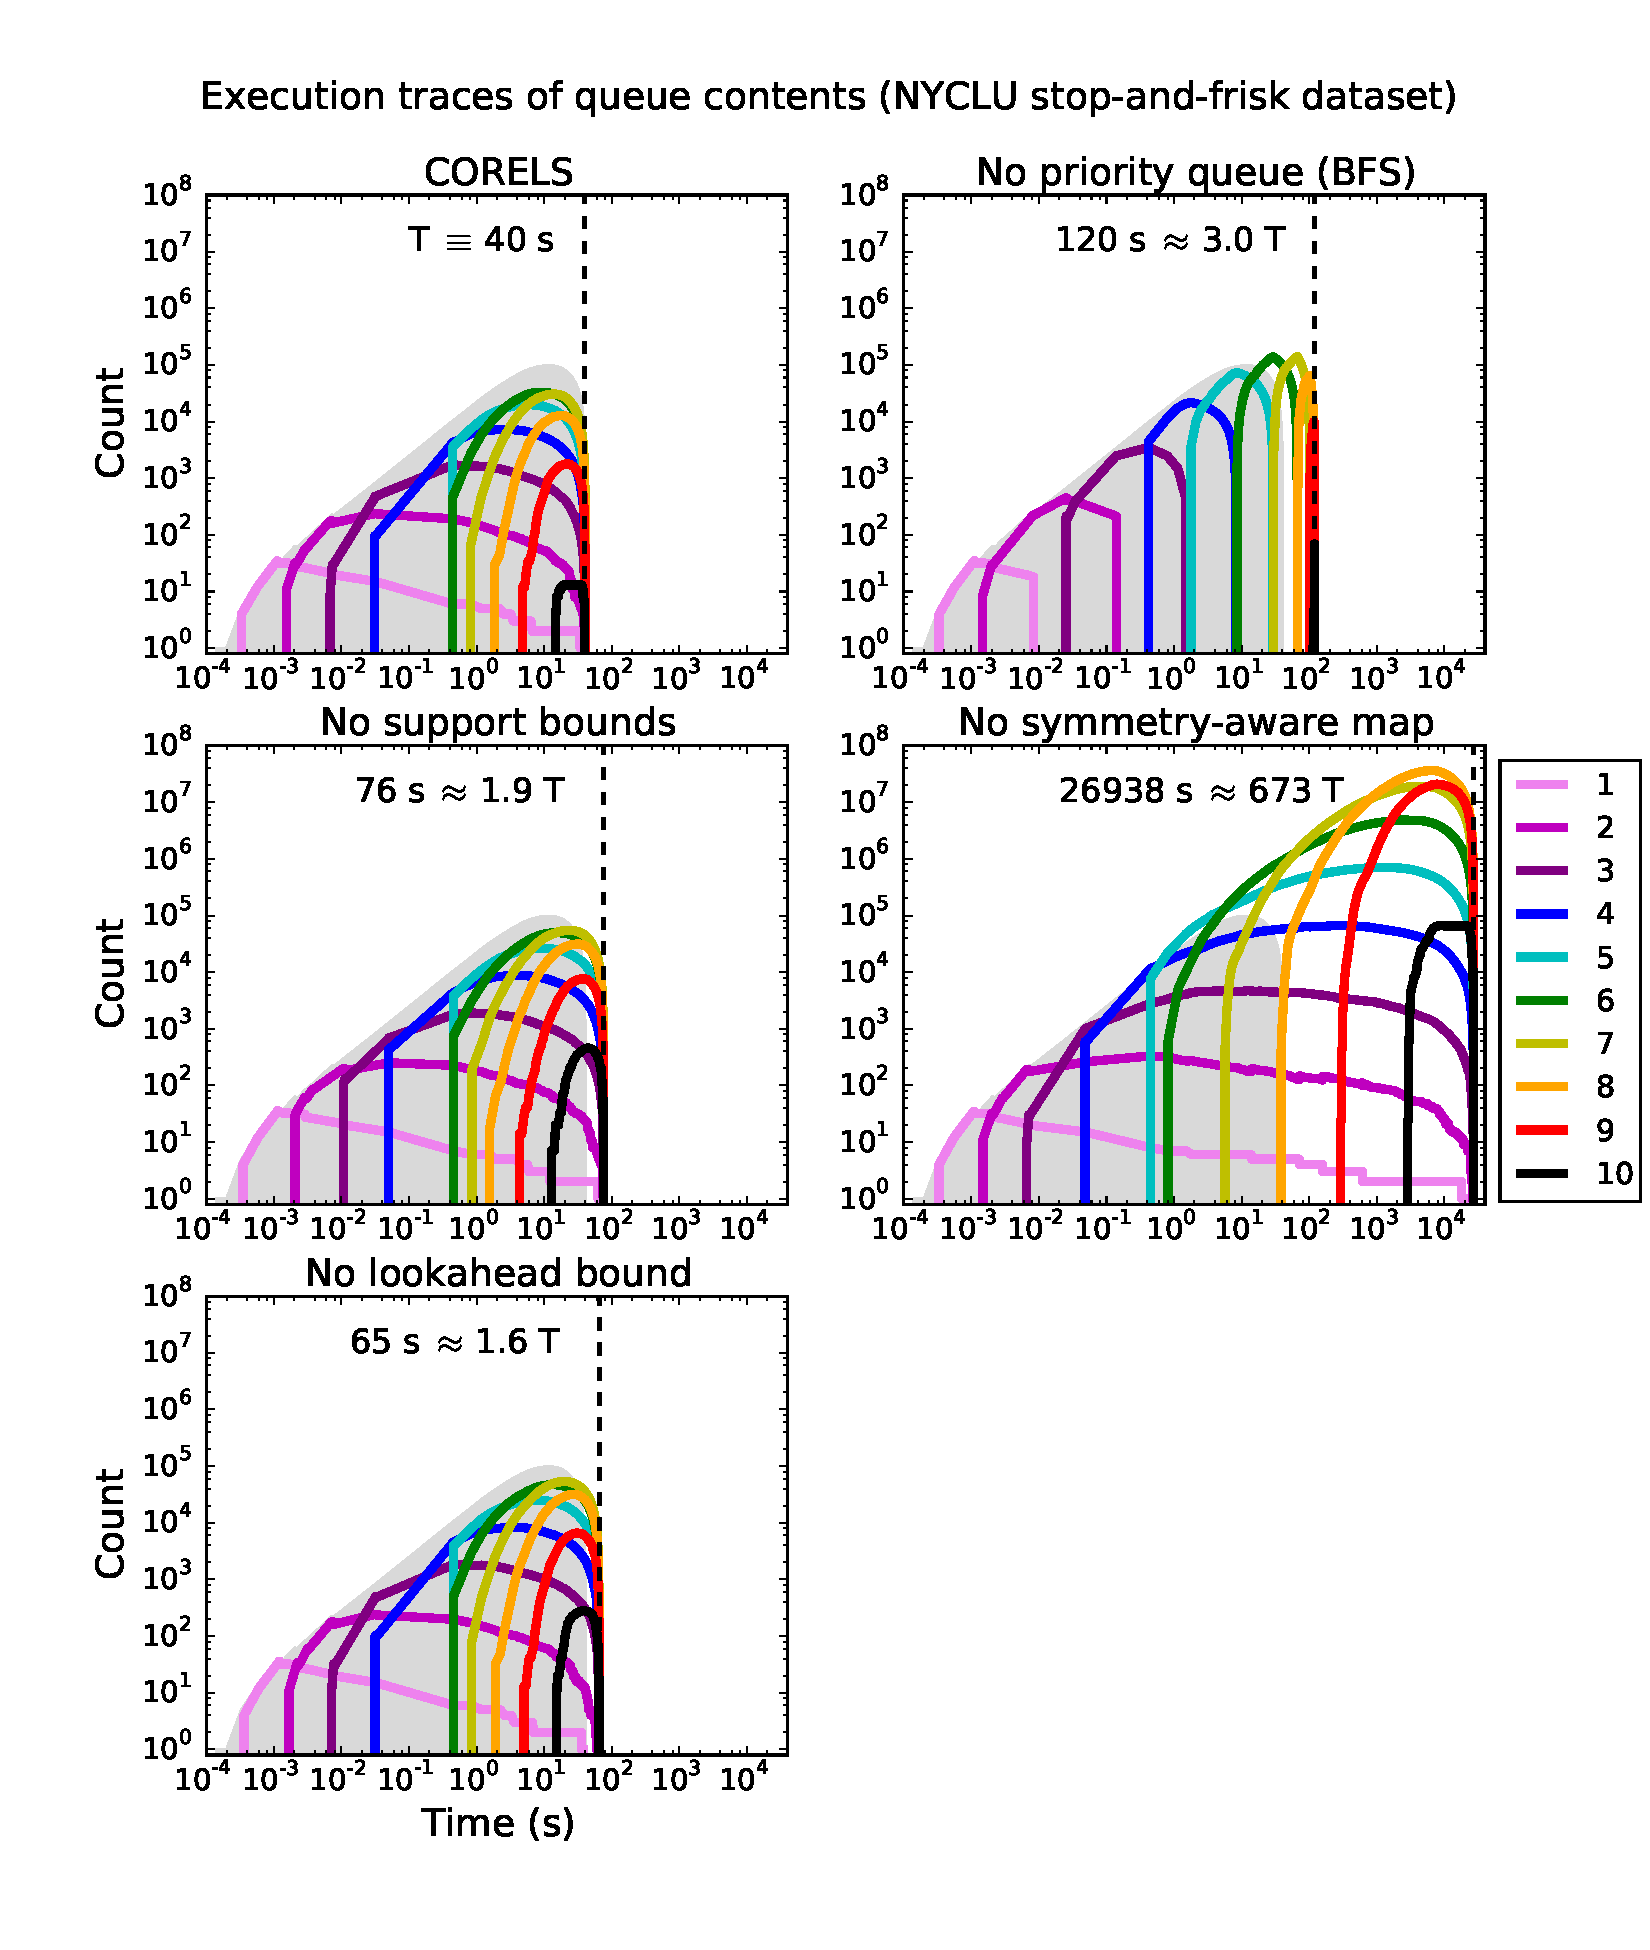
\includegraphics[trim={0mm 0mm 0mm 15mm}, width=\textwidth]{figs/weapon_ablation-queue.pdf}
\end{center}
\vspace{-5mm}
\caption{Summary of the logical queue's contents, for full CORELS (top left)
and five variants that each remove a specific implementation optimization or bound,
for the NYCLU stop-and-frisk dataset (${\Reg = 0.01}$, ${M = 46}$), as in Table~\ref{tab:ablation-weapon}.
The execution without the symmetry-aware map (bottom left) is incomplete.
%
See Figure~\ref{fig:queue} for a detailed caption.
}
\label{fig:queue-weapon}
\end{figure}

Removing any single optimization increases total execution time,
by varying amounts across these optimizations.
%
Similar to our experiments in~\S\ref{sec:reg-param}, we always encounter the
optimal rule list in far less time than it takes to certify optimality.
%
As in Table~\ref{tab:weapon-reg}, we report metrics that are all proxies
for how much computational work our algorithm must perform;
these metrics thus scale with the overall slowdown with respect to CORELS execution time
(Table~\ref{tab:ablation}, first column).

Figure~\ref{fig:queue} visualizes execution traces of the elements in CORELS' logical queue,
similar to Figure~\ref{fig:queue-weapon-reg},
for a single, representative cross-validation fold.
%
Panels correspond to different removed optimizations, as in Table~\ref{tab:ablation}.
%
These plots demonstrate that our optimizations reduce the number of evaluated prefixes
and are especially effective at limiting the number of longer evaluated prefixes.
%
For the ProPublica dataset, the most important optimization is the equivalent points
bound---without it, we place prefixes of at least length~10 in our queue,
and must terminate these executions before they are complete.
%
In contrast, CORELS and most other variants evaluate only prefixes up to at most length~5,
except for the variant without the lookahead bound, which evaluates prefixes up to length~6.

Table~\ref{tab:ablation-weapon} and Figure~\ref{fig:queue-weapon} summarize an
analogous set of experiments for the NYCLU dataset.
%
Note that while the equivalent points bound proved to be the most important optimization for the ProPublica dataset,
the symmetry-aware map is the crucial optimization for the NYCLU dataset.

\begin{figure}[t!]
\begin{center}
%\includegraphics[width=0.65\textwidth]{figs/sketch-objective.png}
% left lower right upper
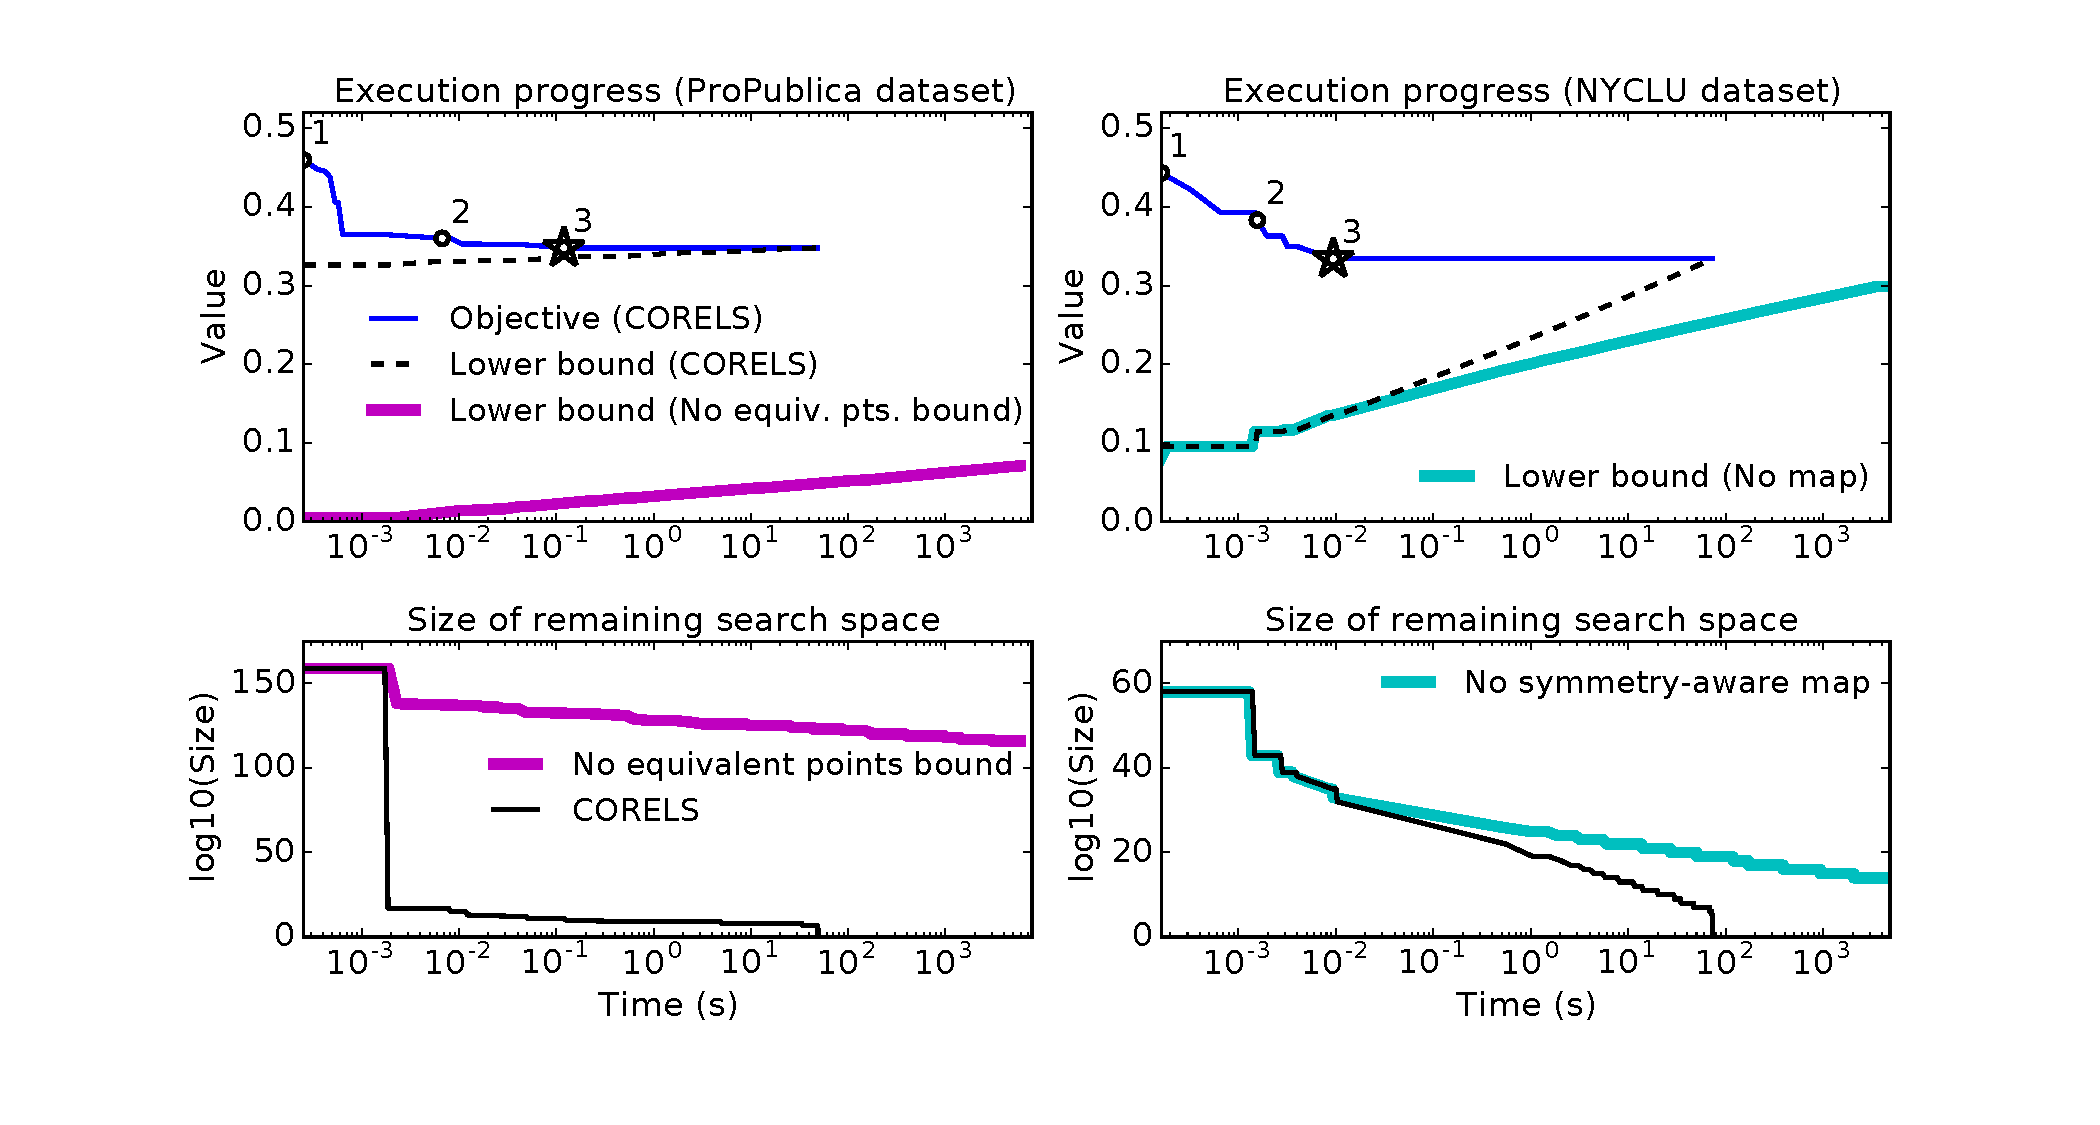
\includegraphics[trim={30mm, 20mm, 30mm, 20mm},
width=0.95\textwidth]{figs/weapon_execution_large-remaining-space.pdf}
\end{center}
\caption{Execution progress of CORELS and selected variants,
for the ProPublica (${\Reg = 0.005}$, ${M = 122}$) (left)
and NYCLU (${\Reg = 0.01}$, ${M = 46}$) (right) datasets.
%
Top: Objective value (thin solid lines) and lower bound (dashed lines) for CORELS,
as a function of wall clock time (log scale).
%
Numbered points along the trace of the objective value
indicate when the length of the best known rule list changes,
and are labeled by the new length.
%
CORELS quickly achieves the optimal value (star markers),
and certifies optimality when the lower bound matches the objective value.
%
On the left, a separate and significantly longer execution of CORELS
without the equivalent points  (Theorem~\ref{thm:identical}) bound remains
far from complete, and its lower bound (thick solid line) far from the optimum.
%
On the right, a separate execution of CORELS without the permutation bound
(Corollary~\ref{thm:permutation}), and thus the symmetry-aware map,
requires orders of magnitude more time to complete.
%
Bottom: $\lfloor \log_{10} \Remaining(\CurrentObj, \Queue) \rfloor$,
as a function of wall clock time (log scale),
where~$\Remaining(\CurrentObj, \Queue)$
is the upper bound~\eqref{eq:remaining} on remaining search space size
(Theorem~\ref{thm:remaining-eval-fine}).
%
For these problems, the equivalent points (left) and
permutation (right) bounds are responsible for the ability of
CORELS to quickly eliminate most of the search space (thin solid lines);
the remaining search space decays much more slowly without these bounds (thick solid lines).
}
\label{fig:objective}
\end{figure}

Finally, Figure~\ref{fig:objective} highlights the most significant
algorithm optimizations for our prediction problems:
the equivalent points bound for the ProPublica dataset (left)
and the symmetry-aware map for the NYCLU dataset (right).
%
For CORELS (thin lines) with the ProPublica recidivism dataset (left),
the objective drops quickly, achieving the optimal value within a second.
CORELS certifies optimality in about a minute---the objective lower bound
steadily converges to the optimal objective (top) as the search space shrinks (bottom).
%
As in Figure~\ref{fig:weapon-reg-execution}, we dynamically and incrementally
calculate~$\lfloor \log_{10} \Remaining(\CurrentObj, \Queue) \rfloor$,
where~$\Remaining(\CurrentObj, \Queue)$
is the upper bound~\eqref{eq:remaining} on remaining search space size
(Theorem~\ref{thm:remaining-eval-fine}); this adds some computational overhead.
%
In the same plots (left), we additionally highlight
a separate execution of CORELS without the equivalent points bound
(Theorem~\ref{thm:identical}) (thick lines).
%
After more than 2 hours, the execution is still far from complete;
in particular, the lower bound is far from the optimum objective value (top)
and much of the search space remains unexplored~(bottom).
%
For the NYCLU stop-and-frisk dataset (right),
CORELS achieves the optimum objective in well under a second,
and certifies optimality in a little over a minute.
%
CORELS without the permutation bound (Corollary~\ref{thm:permutation}),
and thus the symmetry-aware map,
requires more than an hour, \ie orders of magnitude more time, to complete (thick lines).

\subsection{Algorithmic Speedup}
\label{sec:speedup}

\begin{table}[t!]
%\vspace{5mm}
\centering
\begin{tabular}{l|c|c|r l}
Algorithmic & Max evaluated & Lower bound & Predicted&runtime \\
approach & prefix length & evaluations & \\
\hline
CORELS & 5  & $ 2.8 \times 10^7$ & &$36$ seconds \\
Brute force & 5 & ~$2.5 \times 10^{10}$ & $3.3 \times 10^4$ s =&$9.0$ hours \\
Brute force & 10 & ~$5.0 \times 10^{20}$ & $6.5 \times 10^{14}$ s =&$21$ million years \\
CORELS (1984) & 5 & $2.8 \times 10^7$ & $1.2 \times 10^6$ s =&$13.5$ days \\
\end{tabular}
\caption{Algorithmic speedup for the ProPublica dataset (${\Reg = 0.005}$, ${M = 122}$).
%
Solving this problem using brute force is impractical due to the inability to explore rule lists of reasonable lengths.
%
Removing only the equivalent points bound requires exploring prefixes of up to length 10 (see Table \ref{tab:ablation}), a clearly intractable problem.
%
Even with all of our improvements, however, it is only recently that processors have been fast enough in order to allow this type of discrete optimization algorithm to succeed.
}
%\vspace{4mm}
\label{tab:speedup}
\end{table}

Table \ref{tab:speedup} shows the overall speedup of CORELS compared to a na\"ive implementation
and demonstrates the infeasibility of running our algorithm 30 years ago.
%
Consider an execution of CORELS for the ProPublica dataset, with ${M = 122}$ antecedents,
that evaluates prefixes up to length~5 in order to certify optimality (Table~\ref{tab:ablation}).
%
A brute force implementation that na\"ively considers all prefixes of up to length~5
would evaluate ${2.5 \times 10^{10}}$ prefixes.
%
As shown in Figure~\ref{fig:recidivism-all-folds}, the optimal rule list has prefix length~3,
thus the brute force algorithm would identify the optimal rule list.
%
However, for this approach to certify optimality, it would have consider far longer prefixes.
%
Without our equivalent points bound, but with all of our other optimizations,
we evaluate prefixes up to at least length~10
(see Table~\ref{tab:ablation} and Figure~\ref{fig:queue})---thus a brute force algorithm
would have to evaluate prefixes of length~10 or longer.
%
Na\"ively evaluating all prefixes up to length~10 would require looking at ${5.0 \times 10^{20}}$ different prefixes.

However, CORELS examines only 28 million prefixes in total---a reduction of 893 compared to examining
all prefixes up to length~5 and a reduction of ${1.8 \times 10^{13}}$ for the case of length~10.
%
On a laptop, we require about 1.3~$\mu$s to evaluate a single prefix (given by dividing the number of lower bound evaluations by the total time
in Table~\ref{tab:ablation}). 
%
Our runtime is only about 36 seconds, but the na\"ive solutions of examining all prefixes up to
lengths~5 and~10 would take 9 hours and 21 million years, respectively.
%
It is clear that brute force would not scale to larger problems.

We compare our current computing circumstances to those of 1984, the year when CART was published.
%
Moore's law holds that computing power doubled every 18 months from 1984--2006.
%
This is a period of 264 months, which means computing power has gone up by at least a factor of 32,000 since 1984.
%
Thus, even with our algorithmic and data structural improvements,
CORELS would have required over 1.2 million seconds in 1984---an unreasonable amount of time.
%
Our advances are meaningful only because we can run them on a modern system.
%
Combining our algorithmic improvements with the increase in modern processor speeds,
our algorithm runs more than $10^{13}$ times faster than a na\"ive implementation would have in 1984.
%
This helps explain why neither our algorithm, nor other branch-and-bound variants, had been developed before now.
